\subsection{\texorpdfstring{\carbon{}}{13C} sensitivity-enhanced HSQC}
\label{subsec:noah__sehsqc_c}

The first of these is the sensitivity-enhanced HSQC (seHSQC) experiment, which provides up to $2\times$ increased SNR over a standard (echo--antiecho) HSQC.%
\footnote{Since a States HSQC has $\sqrt{2}$ times the SNR of an EA HSQC (as shown in \cref{fig:hsqc_comparison}), this also means that the seHSQC has a $\sqrt{2}$ SNR improvement over a States HSQC. The literature can be somewhat confusing on this point: sometimes the gain in signal is even conflated with the gain in SNR. The clearest exposition I have found is that provided by Kontaxis et al.\autocite{Kontaxis1994JMRSA}}
In the original version of the seHSQC (\cref{fig:sehsqc_po_crk}), developed by Cavanagh, Rance, and Kay (`CRK')\autocite{Palmer1991JMR,Kay1992JACS}, this is accomplished through the so-called \textit{preservation of equivalent pathways} (PEP) technique\autocite{Cavanagh1993ARNMRS}.

\begin{figure}[!htbp]
    \centering
    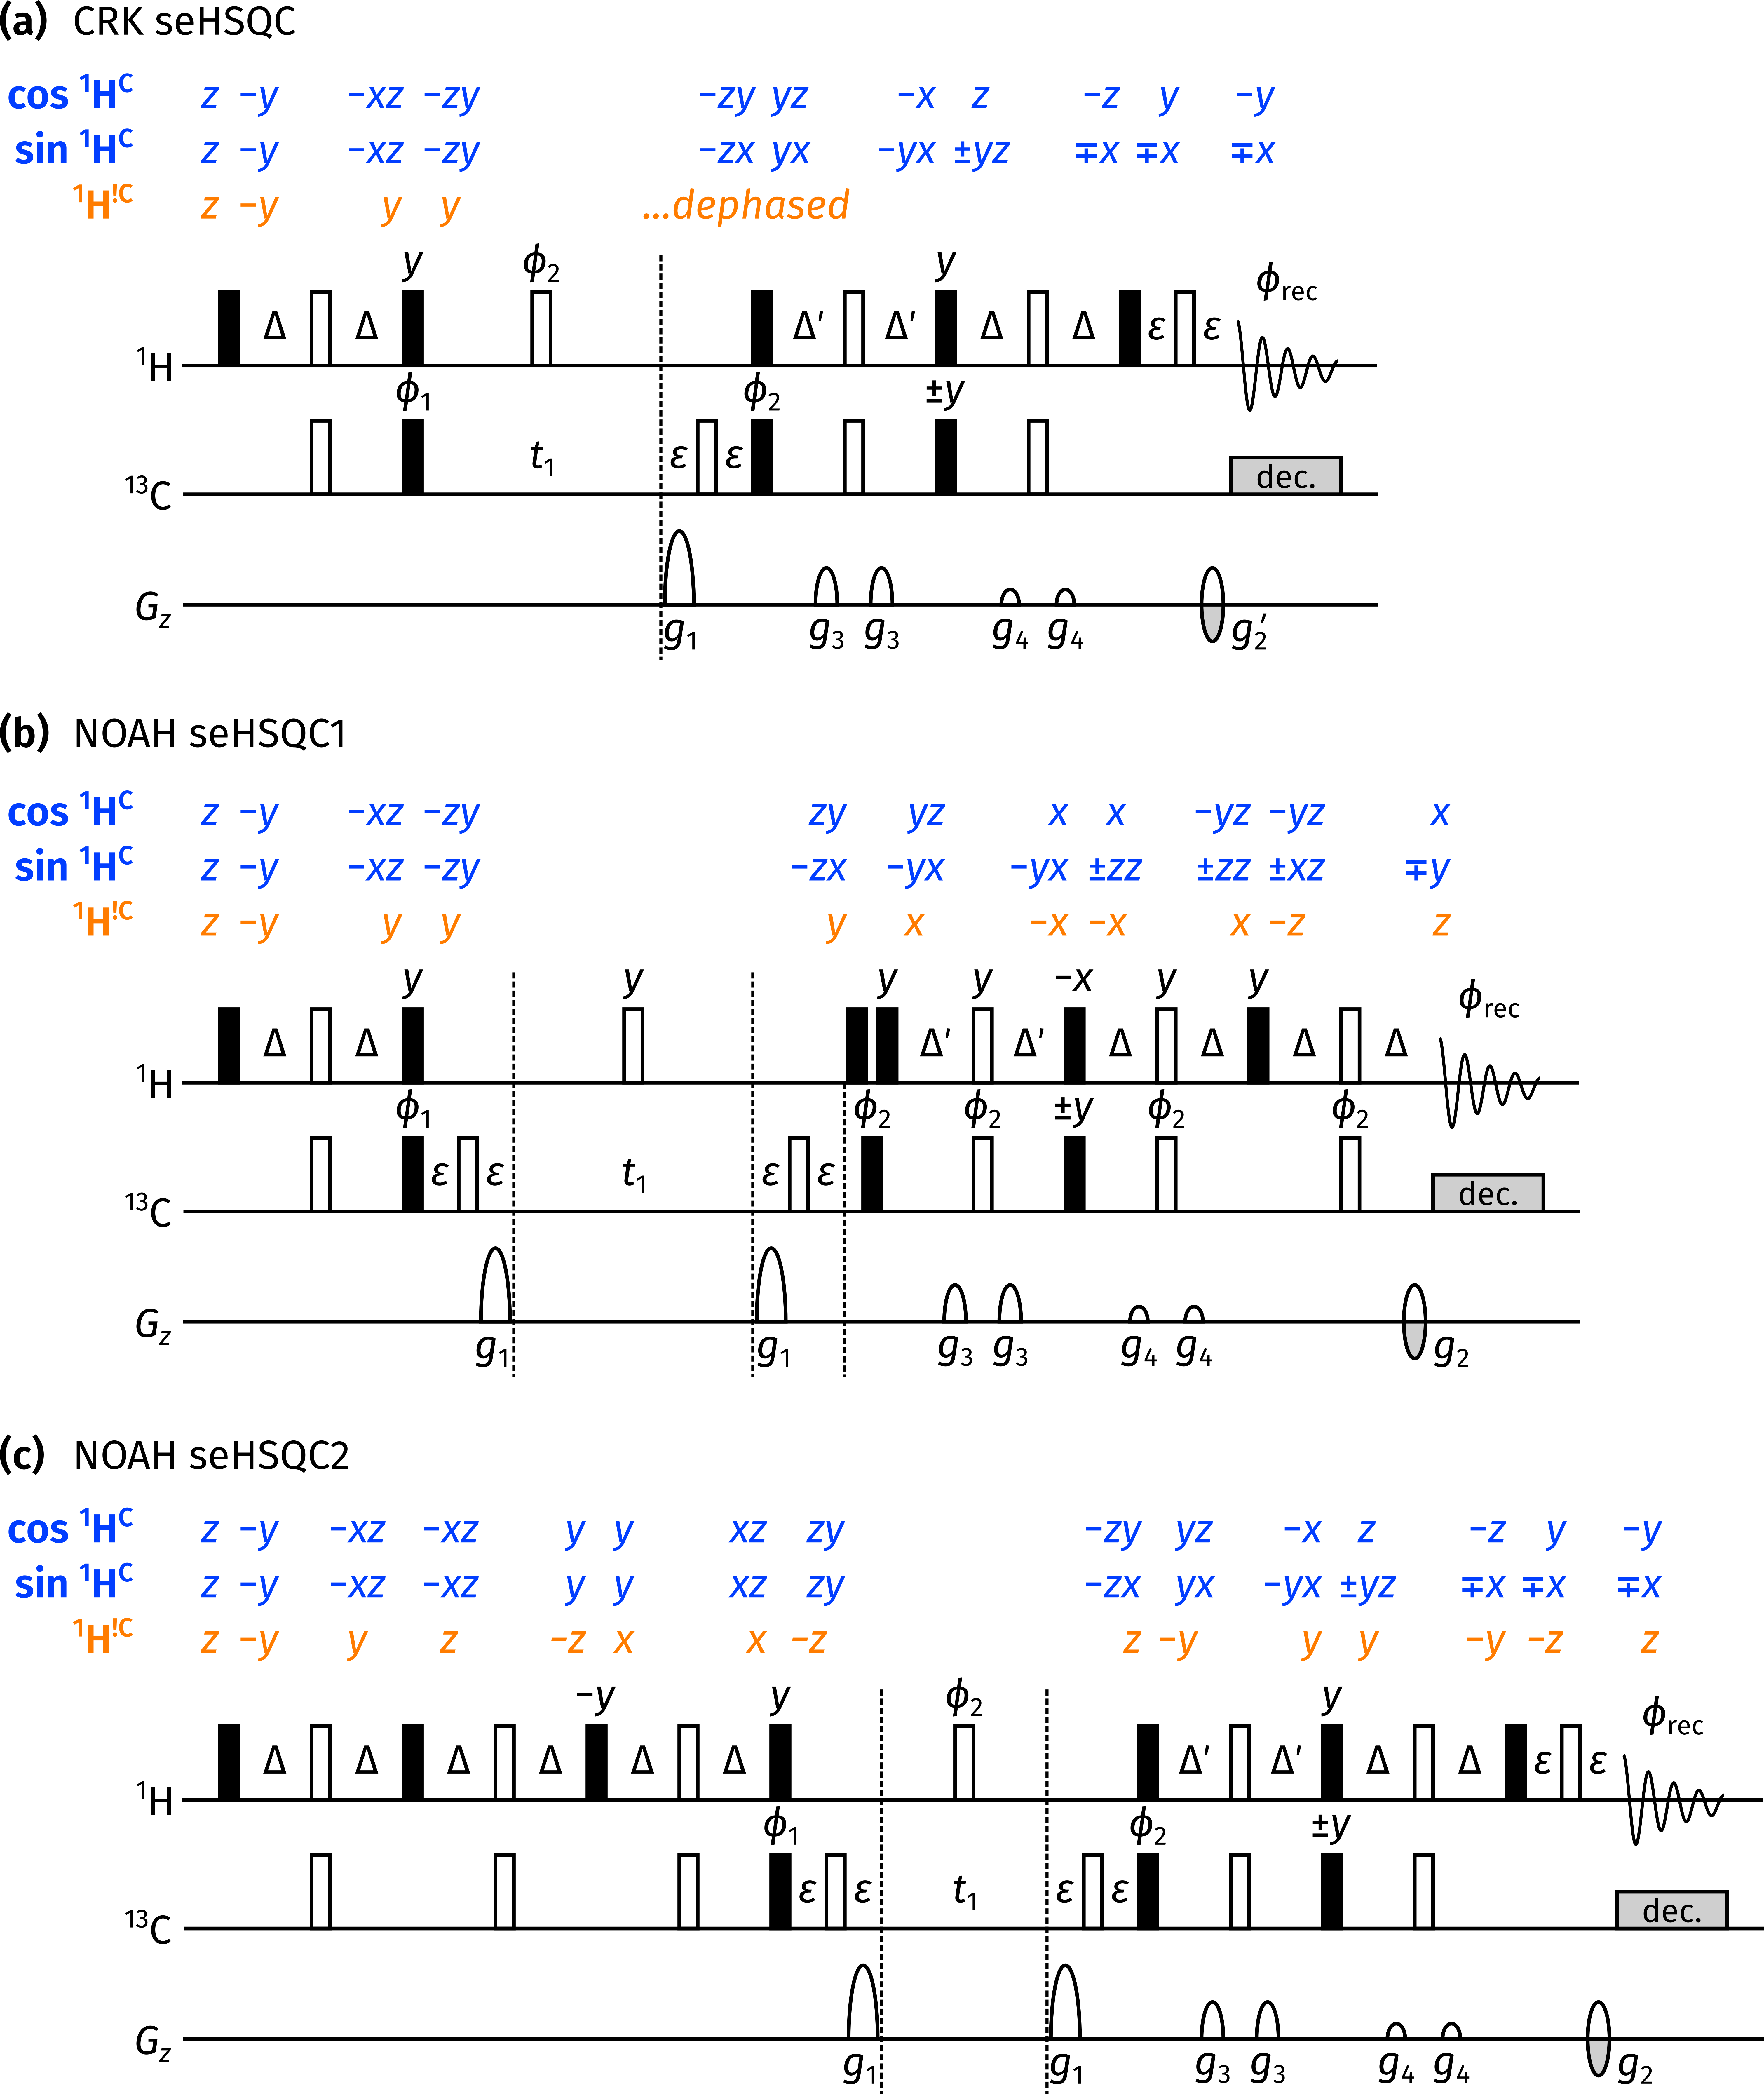
\includegraphics[draft=false]{pp/sehsqc/all_po.png}%
    {\phantomsubcaption\label{fig:sehsqc_po_crk}}%
    {\phantomsubcaption\label{fig:sehsqc_po_noah1}}%
    {\phantomsubcaption\label{fig:sehsqc_po_noah2}}%
    \caption[CRK seHSQC and NOAH seHSQC modules]{
        Sensitivity-enhanced HSQC sequences discussed in this section, along with product operator analysis.
        This analysis is provided only for the first step of the phase cycle, and assumes an $IS\/$ spin pair with $\Delta' = 1 / (4 \cdot \oneJ{CH})$.
        `cos \magn{C}' refers to the component of the \magn{C} magnetisation which is cosine-modulated during $t_1$.
        \textbf{(\subref{fig:sehsqc_po_crk})} Cavanagh--Rance--Kay seHSQC.
        \textbf{(\subref{fig:sehsqc_po_noah1})} NOAH seHSQC1 module.
        \textbf{(\subref{fig:sehsqc_po_noah2})} NOAH seHSQC2 module.
        Phase cycling is performed with $\phi_1 = (x, -x)$, $\phi_2 = (x, x, -x, -x)$, and $\phi_\text{rec} = (x, -x, -x, x)$.
        The delay $\Delta$ is set to $1 / (4 \cdot \oneJ{CH})$; see the text for a discussion of $\Delta'$.
        The pulses marked with a phase of $\pm y$ are applied with a phase of $y$ in the echo experiment and $-y$ in the antiecho.
        Gradient amplitudes are $(g_1, g_2, g_2', g_3, g_4) = (80\%, \pm 40.2\%, \pm 20.1\%, 11\%, -5\%)$.
    }
    \label{fig:sehsqc_po}
\end{figure}

Just like in a standard HSQC, the experiment begins with an INEPT block and $t_1$ evolution.
At the end of $t_1$, there are two terms which are cosine- and sine-modulated with respect to $\Omega_S$.
In the standard HSQC, only the $2I_zS_y$ term is returned into observable \proton{} magnetisation by the reverse INEPT block (see \cref{subsec:theory__hsqc_states}).
In contrast, the PEP block transfers \textit{both} terms back to \proton{} and subsequently detects both.
Specifically, in the echo experiment it accomplishes the transfer $2I_zS_y \to I_y$ and $2I_zS_x \to I_x$, meaning that the density operator at the end of $t_1$
\begin{equation}
    \label{eq:sehsqc_t1_modulation}
    -2I_zS_y \cos(\Omega_S t_1) - 2I_zS_x \sin(\Omega_S t_1)
\end{equation}
is transformed into
\begin{equation}
    \label{eq:sehsqc_before_detection}
    -I_y \cos(\Omega_S t_1) - I_x \sin(\Omega_S t_1)
\end{equation}
just prior to acquisition.
During the FID, only the $-1$-coherence component is detected:
\begin{equation}
    \label{eq:sehsqc_detection_minusone}
    \frac{1}{2\mi}I_- \cos(\Omega_S t_1) - \frac{1}{2}I_- \sin(\Omega_S t_1) = \frac{1}{2\mi}I_-\exp(-\mi \Omega_S t_1),
\end{equation}
yielding a signal of
\begin{equation}
    \label{eq:s_echo_sehsqc}
    \frac{1}{2\mi}\exp(-\mi \Omega_S t_1)\exp(\mi \Omega_I t_2),
\end{equation}
which has a $2\times$ larger amplitude than the original EA HSQC (\cref{eq:hsqc_ea_echo_signal}).
The antiecho experiment can be similarly analysed.
Since the seHSQC has the same noise level as in an EA HSQC, this also corresponds to a $2\times$ increase in SNR.

It should, however, be noted that the PEP transfer is only fully attained for $IS\/$ spin pairs if the delay $\Delta'$ is set to $1 / (4 \cdot \oneJ{CH})$.
For $I_2S\/$ or $I_3\/S$ spin systems, no gain in sensitivity is accomplished with this setting of $\Delta' = 1 / (4 \cdot \oneJ{CH})$.
It is more common, therefore, to shorten $\Delta'$ to $1 / (8 \cdot \oneJ{CH})$: this sacrifices some transfer efficiency for $IS\/$ systems, but allows for some sensitivity enhancement for $I_2S\/$ and $I_3S\/$ systems (\cref{tbl:sehsqc_theory}).

\begin{table}[!ht]
    \begin{tabular}{cccc}
        \toprule
        \textbf{Spin system} & \multicolumn{3}{c}{\textbf{Theoretical sensitivity enhancement}} \\
        \cmidrule(lr){2-4}
                             & $\Delta' = 1 / (4 \cdot \oneJ{CH})$ & $\Delta' = 1 / (8 \cdot \oneJ{CH})$ & $\Delta' = 1 / (12 \cdot \oneJ{CH})$ \\
        \midrule
        $IS$   & 2 & 1.71 & 1.5  \\
        $I_2S$ & 1 & 1.41 & 1.37 \\
        $I_3S$ & 1 & 1.21 & 1.25 \\
        \bottomrule
    \end{tabular}
    \caption[Theoretical sensitivity enhancements in the seHSQC]{
        Theoretical sensitivity enhancements for $IS\/$, $I_2S\/$, and $I_3S\/$ spin systems in the seHSQC, as a function of the delay $\Delta'$.
        The values are taken from Schleucher et al.\autocite{Schleucher1994JBNMR}
    }
    \label{tbl:sehsqc_theory}
\end{table}


\subsubsection{NOAH seHSQC versions}

Just like the original EA HSQC (\cref{fig:hsqc_etgp}), the CRK seHSQC must be modified in order to be compatible with NOAH supersequences.
In particular, the CTP gradients in the CRK seHSQC dephase the bulk \magnnot{C} magnetisation pool: we would very much like it to return that to $+z$ instead, so that it can be sampled in later homonuclear modules (or, indeed, a HMBC module).
This experiment is more tricky to adapt than the HSQC, because there are \textit{three} different magnetisation components to juggle: the cosine-modulated \magn{C}, sine-modulated \magn{C}, and \magnnot{C}.
Nevertheless, there are at least two ways of doing so; these two modified modules are labelled seHSQC1 and seHSQC2 respectively.

The seHSQC1 module (\cref{fig:sehsqc_po_noah1}) was developed by me.\footnote{Through a great deal of trial and error, and certainly \textit{not} intelligent design.}
It retains the same general structure of the CRK seHSQC up until $t_1$, but immediately after $t_1$ a composite \proton{} pulse is used to effect the transformations
\begin{equation}
    \label{eq:sehsqc1_dp}
    I_z \to I_y; \qquad I_y \to I_x,
\end{equation}
where the former is required for the \magn{C} pool and the latter for \magnnot{C}.
This has the effect of storing the sine-modulated term as $2I_zS_z$ magnetisation for one spin echo (as opposed to the CRK seHSQC, which stores cosine-modulated term as $I_z$).
At the beginning of the final spin echo (containing the rephasing gradient), this is transformed into antiphase magnetisation of the form $2I_xS_z$; thus, this spin echo must be lengthened to a total duration of $2\Delta$ in order to fully refocus $\oneJ{CH}$.
The final modification involves the addition of an extra gradient immediately before to $t_1$: this ensures that the bulk \magnnot{C} magnetisation is not dephased, just like in the NOAH HSQC module (\cref{fig:noah_sb_po_s}).

The seHSQC2 module (\cref{fig:sehsqc_po_noah2}), on the other hand, was initially reported by Hansen et al.\autocite{Hansen2021AC}
In this pulse sequence, the initial \proton{} \ang{90} excitation pulse is replaced with a $zz$ isotope-selective pulse element (ZIP element), which is very similar to the $zz$-filter but has different pulse phases.
This acts as a 90\rlap{\unit{\degree}}$_{-x}$ pulse on the \magn{C} magnetisation pool and thus ultimately leads to the same signals being detected (save for a trivial \ang{180} phase shift).
However, on \magnnot{C} magnetisation, the ZIP element acts as a 90\rlap{\unit{\degree}}$_{y}$ pulse; it turns out that this modification alone is sufficient to return the bulk \magnnot{C} magnetisation to $+z$ at the end of the sequence.
The ZIP element therefore represents an isotope-specific rotation on \proton{} spins, where the rotation axis depends on whether it is coupled to \carbon{} or not.

\begin{figure}[!ht]
    \centering
    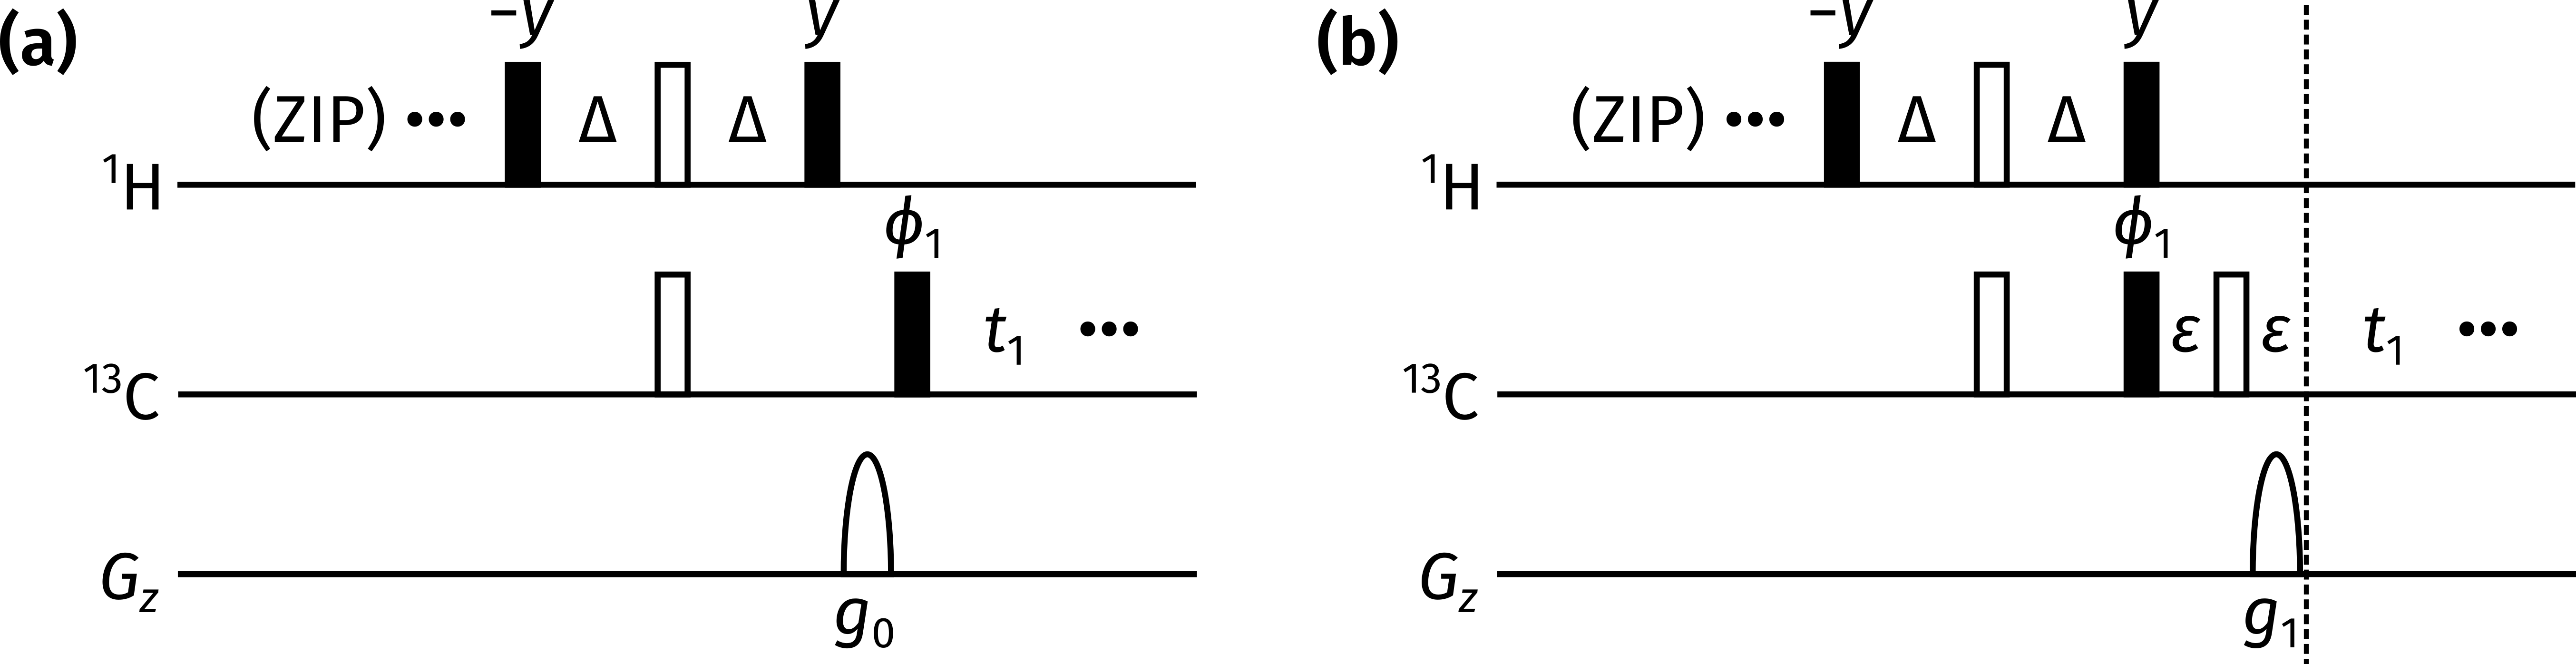
\includegraphics[draft=false]{pp/sehsqc/grad_schemes.png}%
    {\phantomsubcaption\label{fig:sehsqc_grad_schemes_alex}}%
    {\phantomsubcaption\label{fig:sehsqc_grad_schemes_jon}}%
    \caption[Comparison of gradient schemes in seHSQC2 module]{
        Comparison of CTP gradient schemes in seHSQC2 module.
        \textbf{(\subref{fig:sehsqc_grad_schemes_alex})} As reported in Hansen et al.\autocite{Hansen2021AC} $g_0$ is a purge gradient with arbitrary amplitude; the amplitude of the final CTP gradient must be halved.
        \textbf{(\subref{fig:sehsqc_grad_schemes_jon})} The version used in this work (corresponding to \cref{fig:sehsqc_po_noah2}).
    }
    \label{fig:sehsqc_grad_schemes}
\end{figure}

In my work, I made one change to the experiment, namely the addition of an extra gradient echo prior to $t_1$ (thus leading to a symmetric gradient scheme similar to that in seHSQC1).
Instead of this, the original paper had in fact inserted a purge gradient between the \proton{} and \carbon{} \ang{90} pulses just after the INEPT spin echo (\cref{fig:sehsqc_grad_schemes}).
The scheme I used leads to similar results, but has one advantage in that it allows the amplitude of the final CTP gradient ($g_2$ in \cref{fig:sehsqc_po}) to be twice as large: this is particularly relevant to \nitrogen{} experiments, as will be discussed in \cref{subsec:noah__hmqc}.

\begin{figure}[!ht]
    \centering
    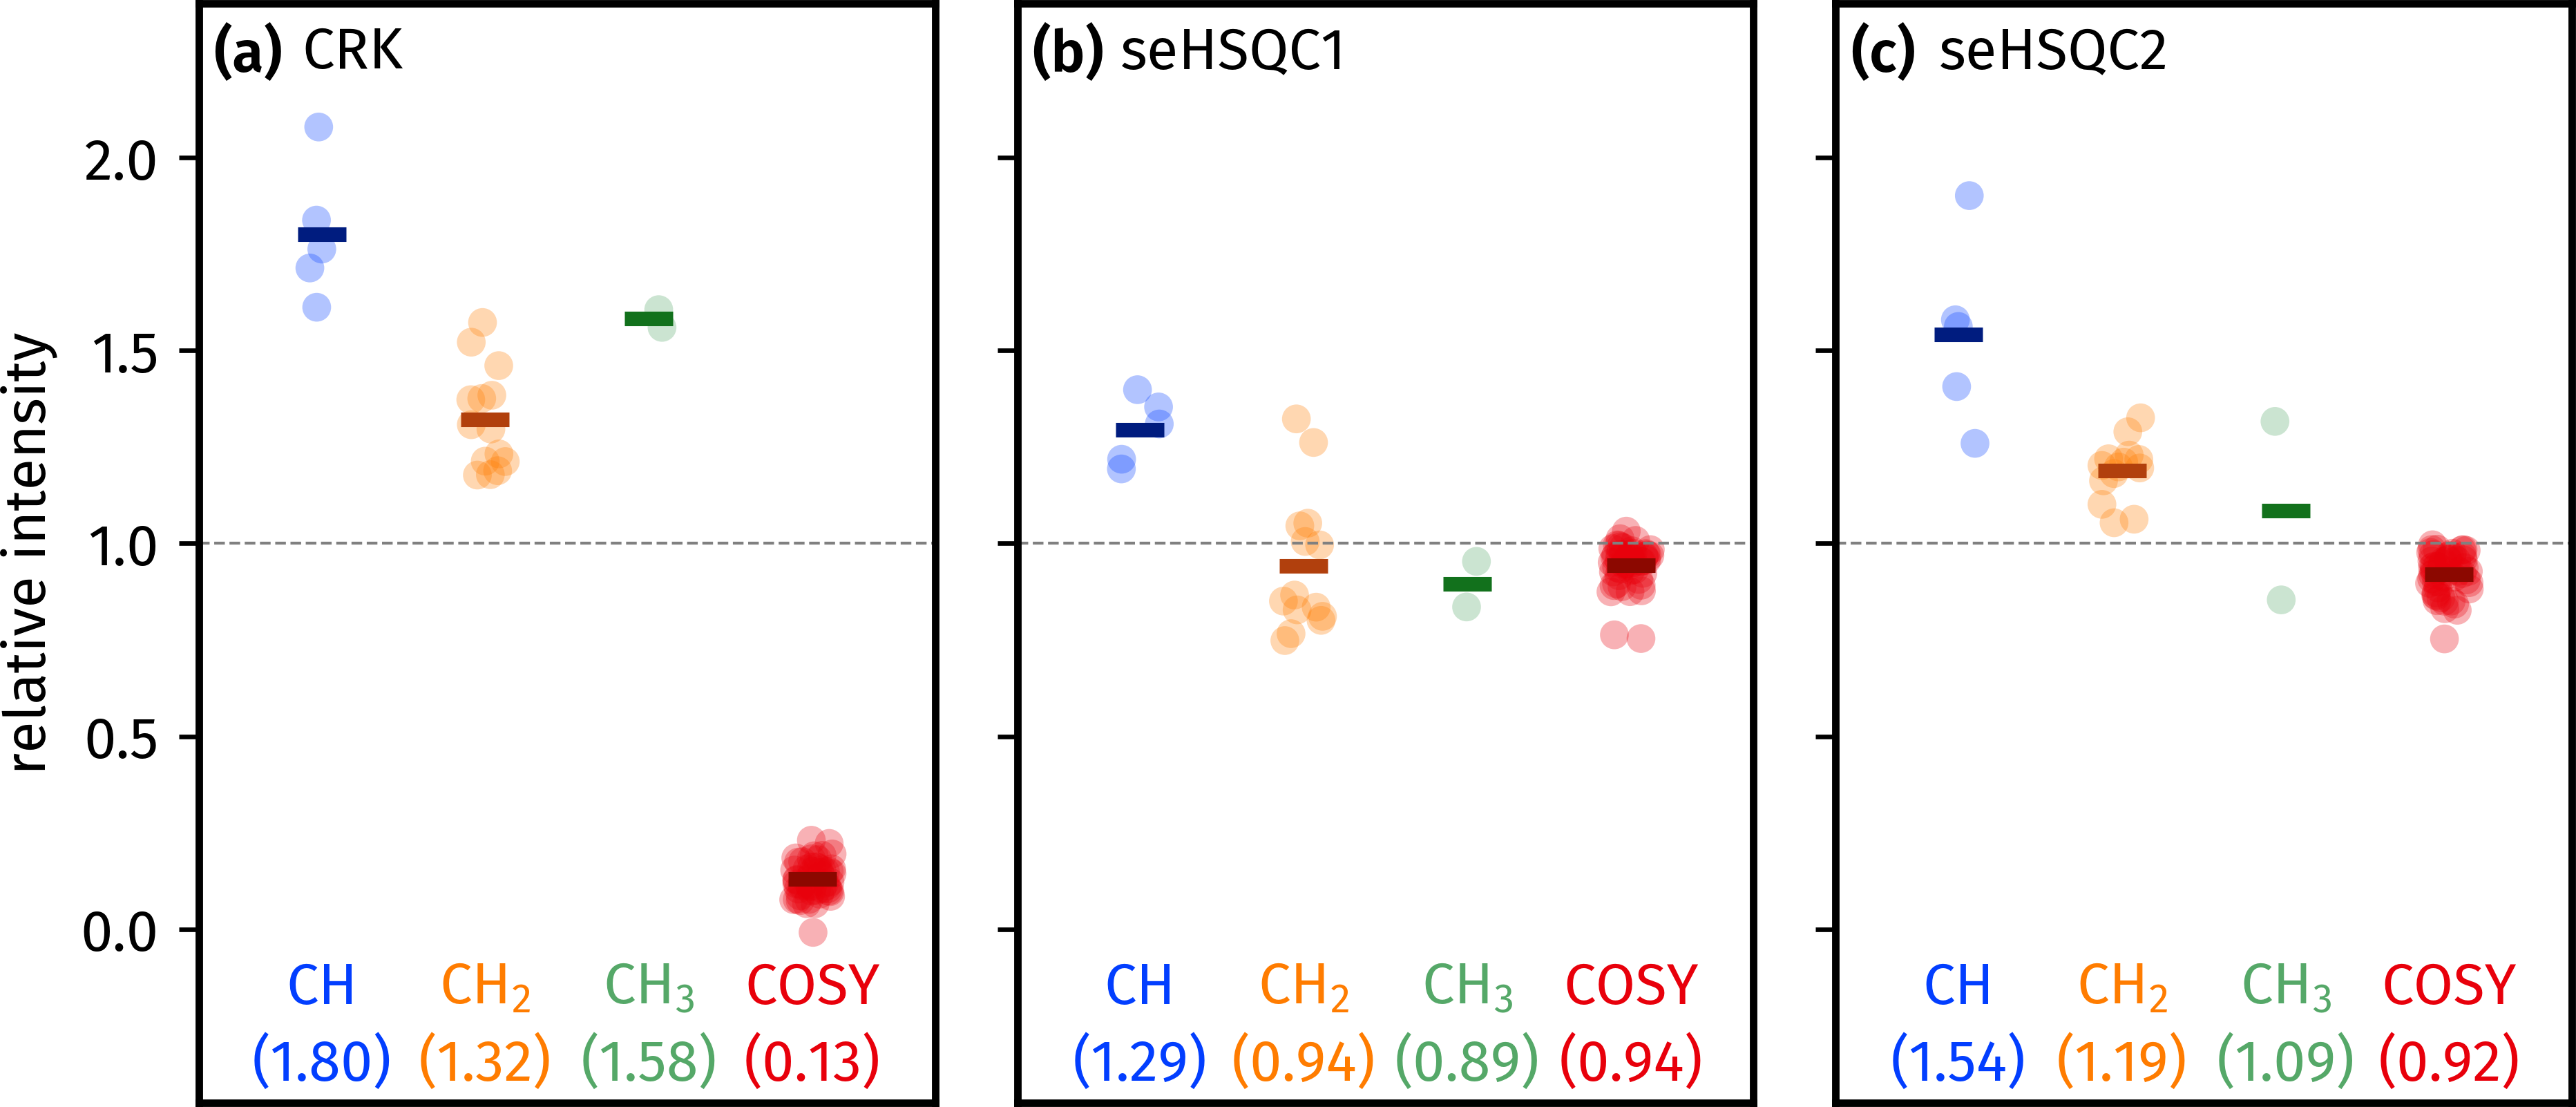
\includegraphics[draft=false]{noah/sehsqc_comp.png}%
    {\phantomsubcaption\label{fig:noah_sehsqc_comp_crk}}%
    {\phantomsubcaption\label{fig:noah_sehsqc_comp_v1}}%
    {\phantomsubcaption\label{fig:noah_sehsqc_comp_v2}}%
    \caption[Comparison of \noah{Sp,Cc} sensitivities]{
        Sensitivities of seHSQC and CLIP-COSY modules in the \noah{Sp,Cc} supersequences (run using $\Delta' = 1 / (8 \cdot \oneJ{CH})$).
        Intensities are reported relative to the corresponding peaks in a \noah{S,Cc} supersequence; HSQC peaks are further broken down by their multiplicity.
        Each dot represents one peak; the solid lines as well as the numbers at the bottom of each plot represent averages over all peaks.
        \textbf{(\subref{fig:noah_sehsqc_comp_crk})} Using the CRK seHSQC.
        \textbf{(\subref{fig:noah_sehsqc_comp_v1})} Using the seHSQC1 module.
        \textbf{(\subref{fig:noah_sehsqc_comp_v2})} Using the seHSQC2 module.
        \datacode{7A-201115}
    }
    \label{fig:noah_sehsqc_comp}
\end{figure}

The primary consideration when evaluating the different seHSQC versions in \cref{fig:sehsqc_po} is naturally sensitivity
\Cref{fig:noah_sehsqc_comp} compares the sensitivities of the various possible \noah{Sp,Cc} supersequence against a \noah{S,Cc} experiment.
As can be seen, all three seHSQC implementations yield improvements in the sensitivities of \ch{CH} peaks: the original CRK seHSQC has the largest effect here, followed by seHSQC2 and seHSQC1.
For \ch{CH2} and \ch{CH3} peaks, the CRK seHSQC and seHSQC2 perform better than the standard HSQC, but the average sensitivities in seHSQC1 have dipped slightly below.
This is not entirely surprising in light of the discussion in \cref{subsec:noah__snr}: the modified seHSQC1 and seHSQC2 sequences are expected to have lower sensitivities than the original experiment from which they are derived.
In this case, it appears that the modifications made to the seHSQC1 sequence have caused sensitivity losses which outweigh the benefits of using a sensitivity-enhanced experiment.

In the context of a NOAH supersequence, it is also important to consider how well each module preserves \magnnot{C} magnetisation for subsequent homonuclear module(s).
In \cref{fig:noah_sehsqc_comp}, the CLIP-COSY module is used as the `reporter' module, but the conclusions drawn here are applicable to \textit{any} homonuclear module (or HMBC).
The CRK seHSQC naturally does poorly in this respect, as it dephases the bulk magnetisation: this leads to almost an order-of-magnitude sensitivity loss in the CLIP-COSY.
Both the other NOAH seHSQC modules, however, perform almost identically to the original HSQC module, as expected from the product operator analysis in \cref{fig:sehsqc_po}.

From \cref{fig:noah_sehsqc_comp}, we can draw some very simple conclusions: if the seHSQC is to be used at (or near) the \textit{beginning} of a NOAH supersequence, where it needs to preserve \magnnot{C} magnetisation, then the seHSQC2 module is the best choice.
On the other hand, if the seHSQC module is placed at the \textit{end} (say in a \noah{B,Sp} supersequence), then the CRK seHSQC is optimal.
This logic is encoded in GENESIS.


\subsubsection{COSY-type artefacts}

One (minor) way in which the seHSQC1 module outperforms seHSQC2 is in the suppression of COSY-type artefacts in the seHSQC spectrum\autocite{Turner1999JMR}.
These arise due to evolution of $\nJ{HH}$ during the second-last spin echo of the CRK seHSQC.
Specifically, if we assume the presence of a separate \proton{} spin $K$ which is coupled to spin $I$, the sine-modulated $2I_yS_z$ term can evolve under both $\oneJ{$IS$}$ and $\nJ{$IK$}$ into $2I_yK_z$, and the last \proton{} \ang{90} pulse transfers this coherence to the spin $K$.
This leads to peaks correlating spin $S$ with $K$.
This is also true of the seHSQC2 module, as the product operator analysis for the CRK seHSQC is entirely applicable to it.

However, for the seHSQC1 module, the corresponding term giving rise to these artefacts would be the cosine-modulated $I_x$ term (at the beginning of the second-last spin echo).
During this spin echo, this can again evolve under both J-couplings into $4I_yK_zS_z$, and the final \ang{90} pulse would transform this to $-4I_zK_yS_z$.
However, crucially, this term is antiphase with respect to the heteronucleus $S$: therefore, when decoupling is applied during acquisition, this term should not be observed.
This analysis can be verified experimentally by inspection of the seHSQC spectra thus obtained.
The COSY-type artefacts, labelled with red boxes in the seHSQC2 spectrum (\cref{fig:sehsqc_cosy_arts_2}), are largely absent in the seHSQC1 spectrum (\cref{fig:sehsqc_cosy_arts_1}).
Some artefacts still remain, which perhaps arise due to pulse imperfections (or perhaps more complicated spin systems than the three-spin system considered here; I did not analyse this in any further detail).

\begin{figure}[!ht]
    \centering
    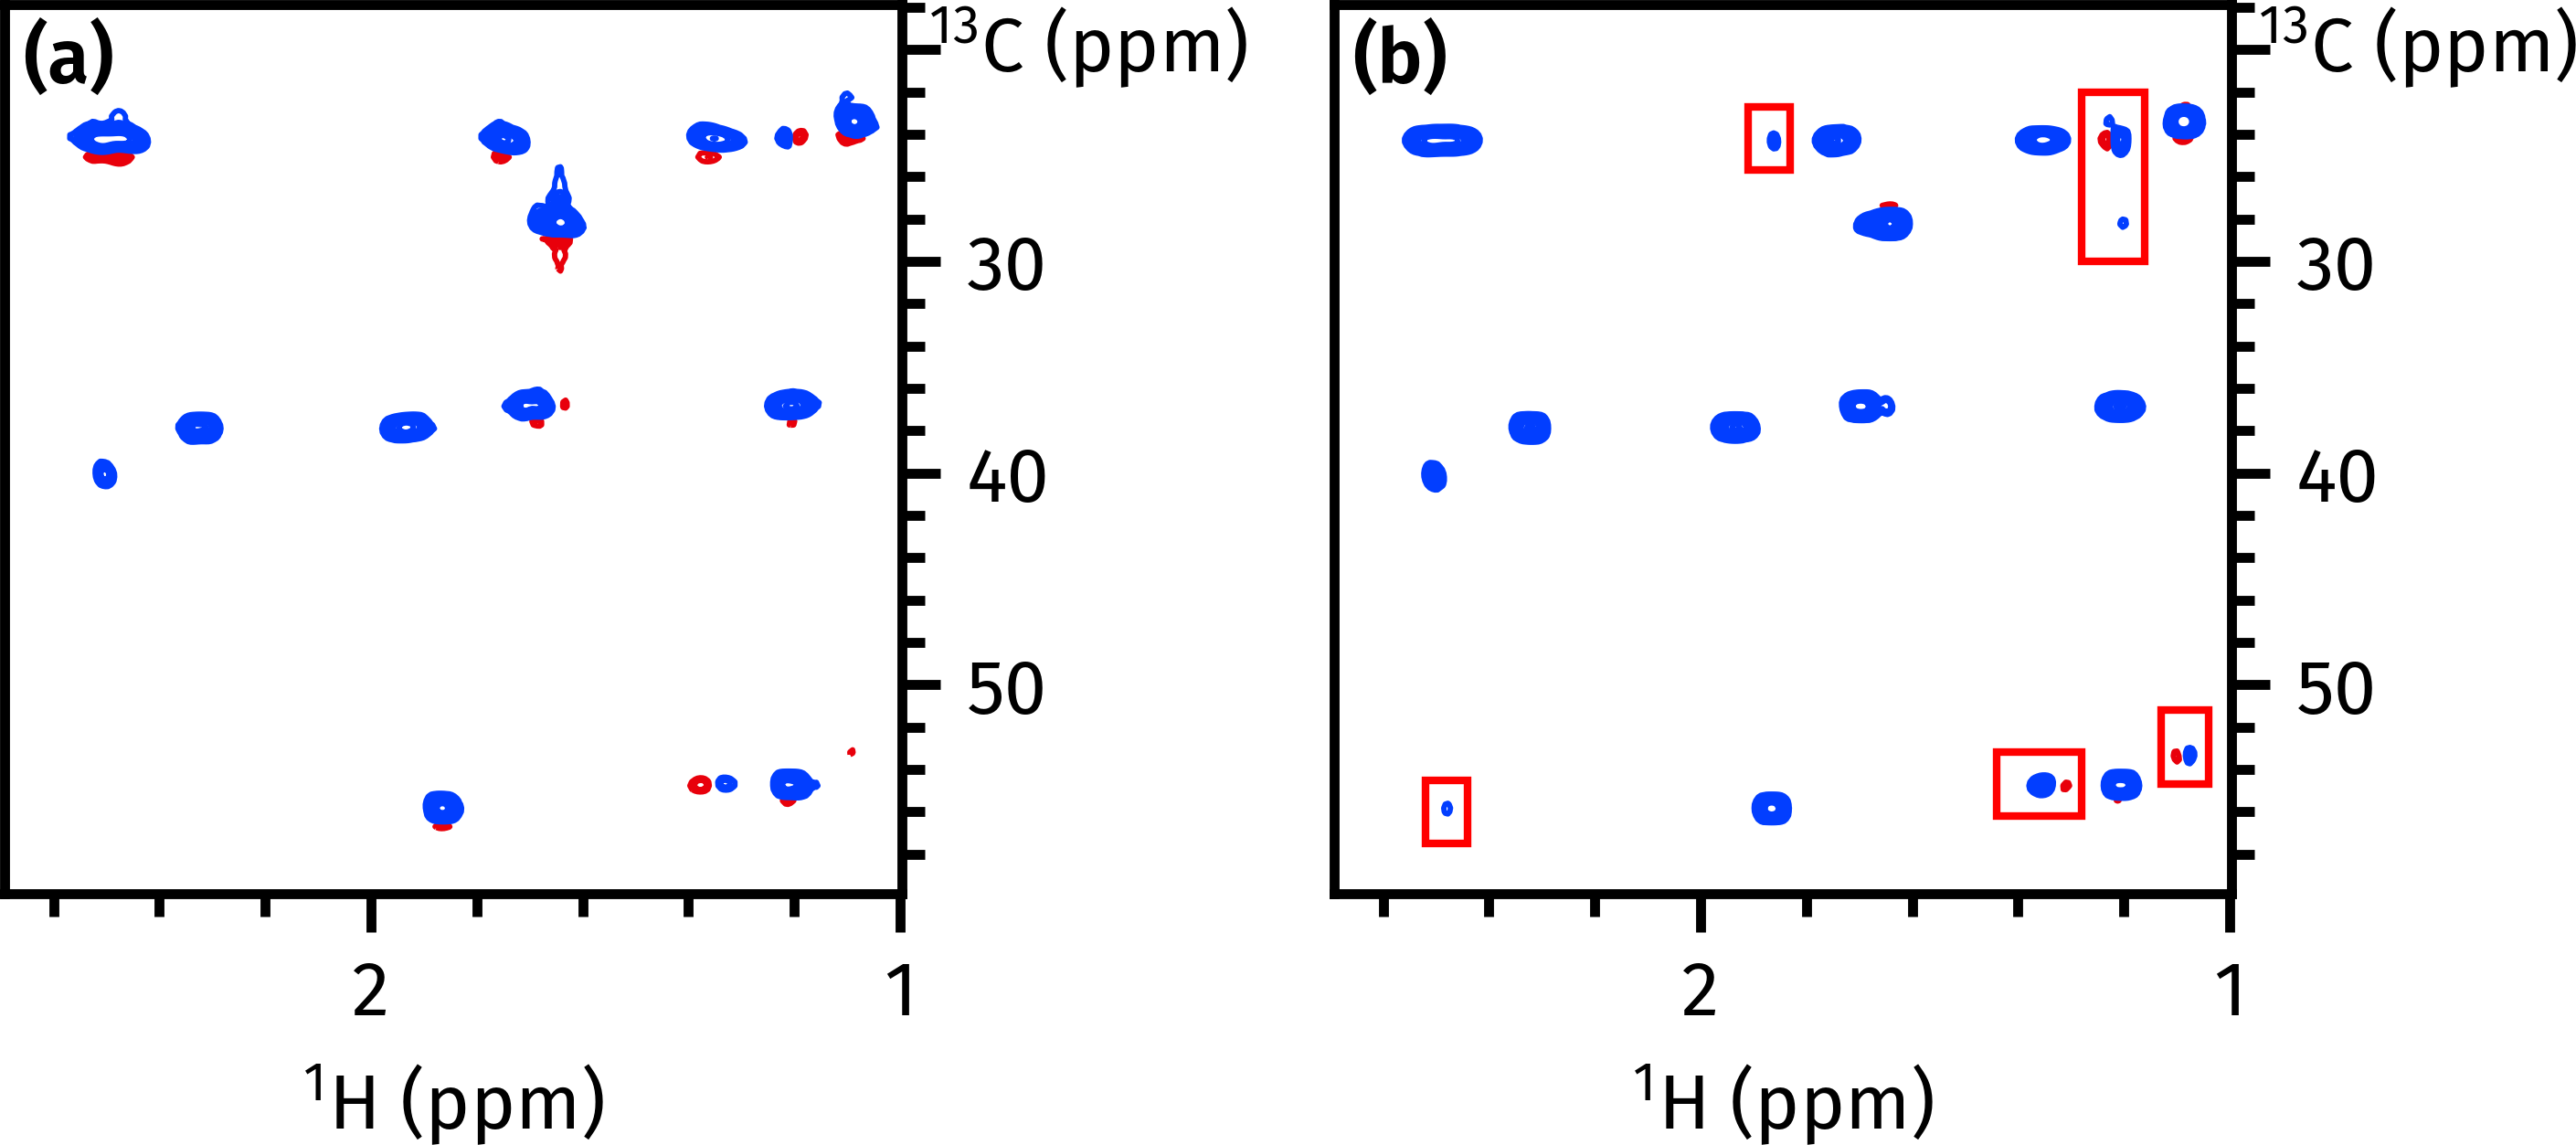
\includegraphics[draft=false]{noah/sehsqc_cosy_arts.png}%
    {\phantomsubcaption\label{fig:sehsqc_cosy_arts_1}}%
    {\phantomsubcaption\label{fig:sehsqc_cosy_arts_2}}%
    \caption[Comparison of COSY-type artefacts in NOAH seHSQC modules]{
        Comparison of COSY-type artefacts in NOAH seHSQC modules.
        \textbf{(\subref{fig:sehsqc_cosy_arts_1})} seHSQC1.
        \textbf{(\subref{fig:sehsqc_cosy_arts_2})} seHSQC2. The artefacts are highlighted in red boxes.
        \datacode{7A-201115}
    }
    \label{fig:sehsqc_cosy_arts}
\end{figure}


\subsubsection{Wing artefacts}

One point worth considering is whether the extra gradient in the seHSQC2 module is truly needed.
In the HSQC and seHSQC1 modules, the bulk magnetisation is placed along the transverse axis during $t_1$; therefore, if a pair of symmetric gradients are not used, this magnetisation will be dephased (as in the CRK seHSQC).
However, in the seHSQC2 module, the bulk magnetisation is longitudinal, which suggests that this gradient is not necessary.

This gradient can indeed be removed in the seHSQC2 module, and doing so does not lead to any poorer preservation of \magnnot{C} magnetisation.
However, the omission of this gradient leads to artefacts in the CLIP-COSY spectrum, which I term \textit{`wing artefacts'} because of the way they flank peaks in the CLIP-COSY (\cref{fig:sehsqc_wing_arts}).
These artefacts can most clearly be seen in the diagonal peaks of methyl groups, but are present across the entire spectrum.

\begin{figure}[!ht]
    \centering
    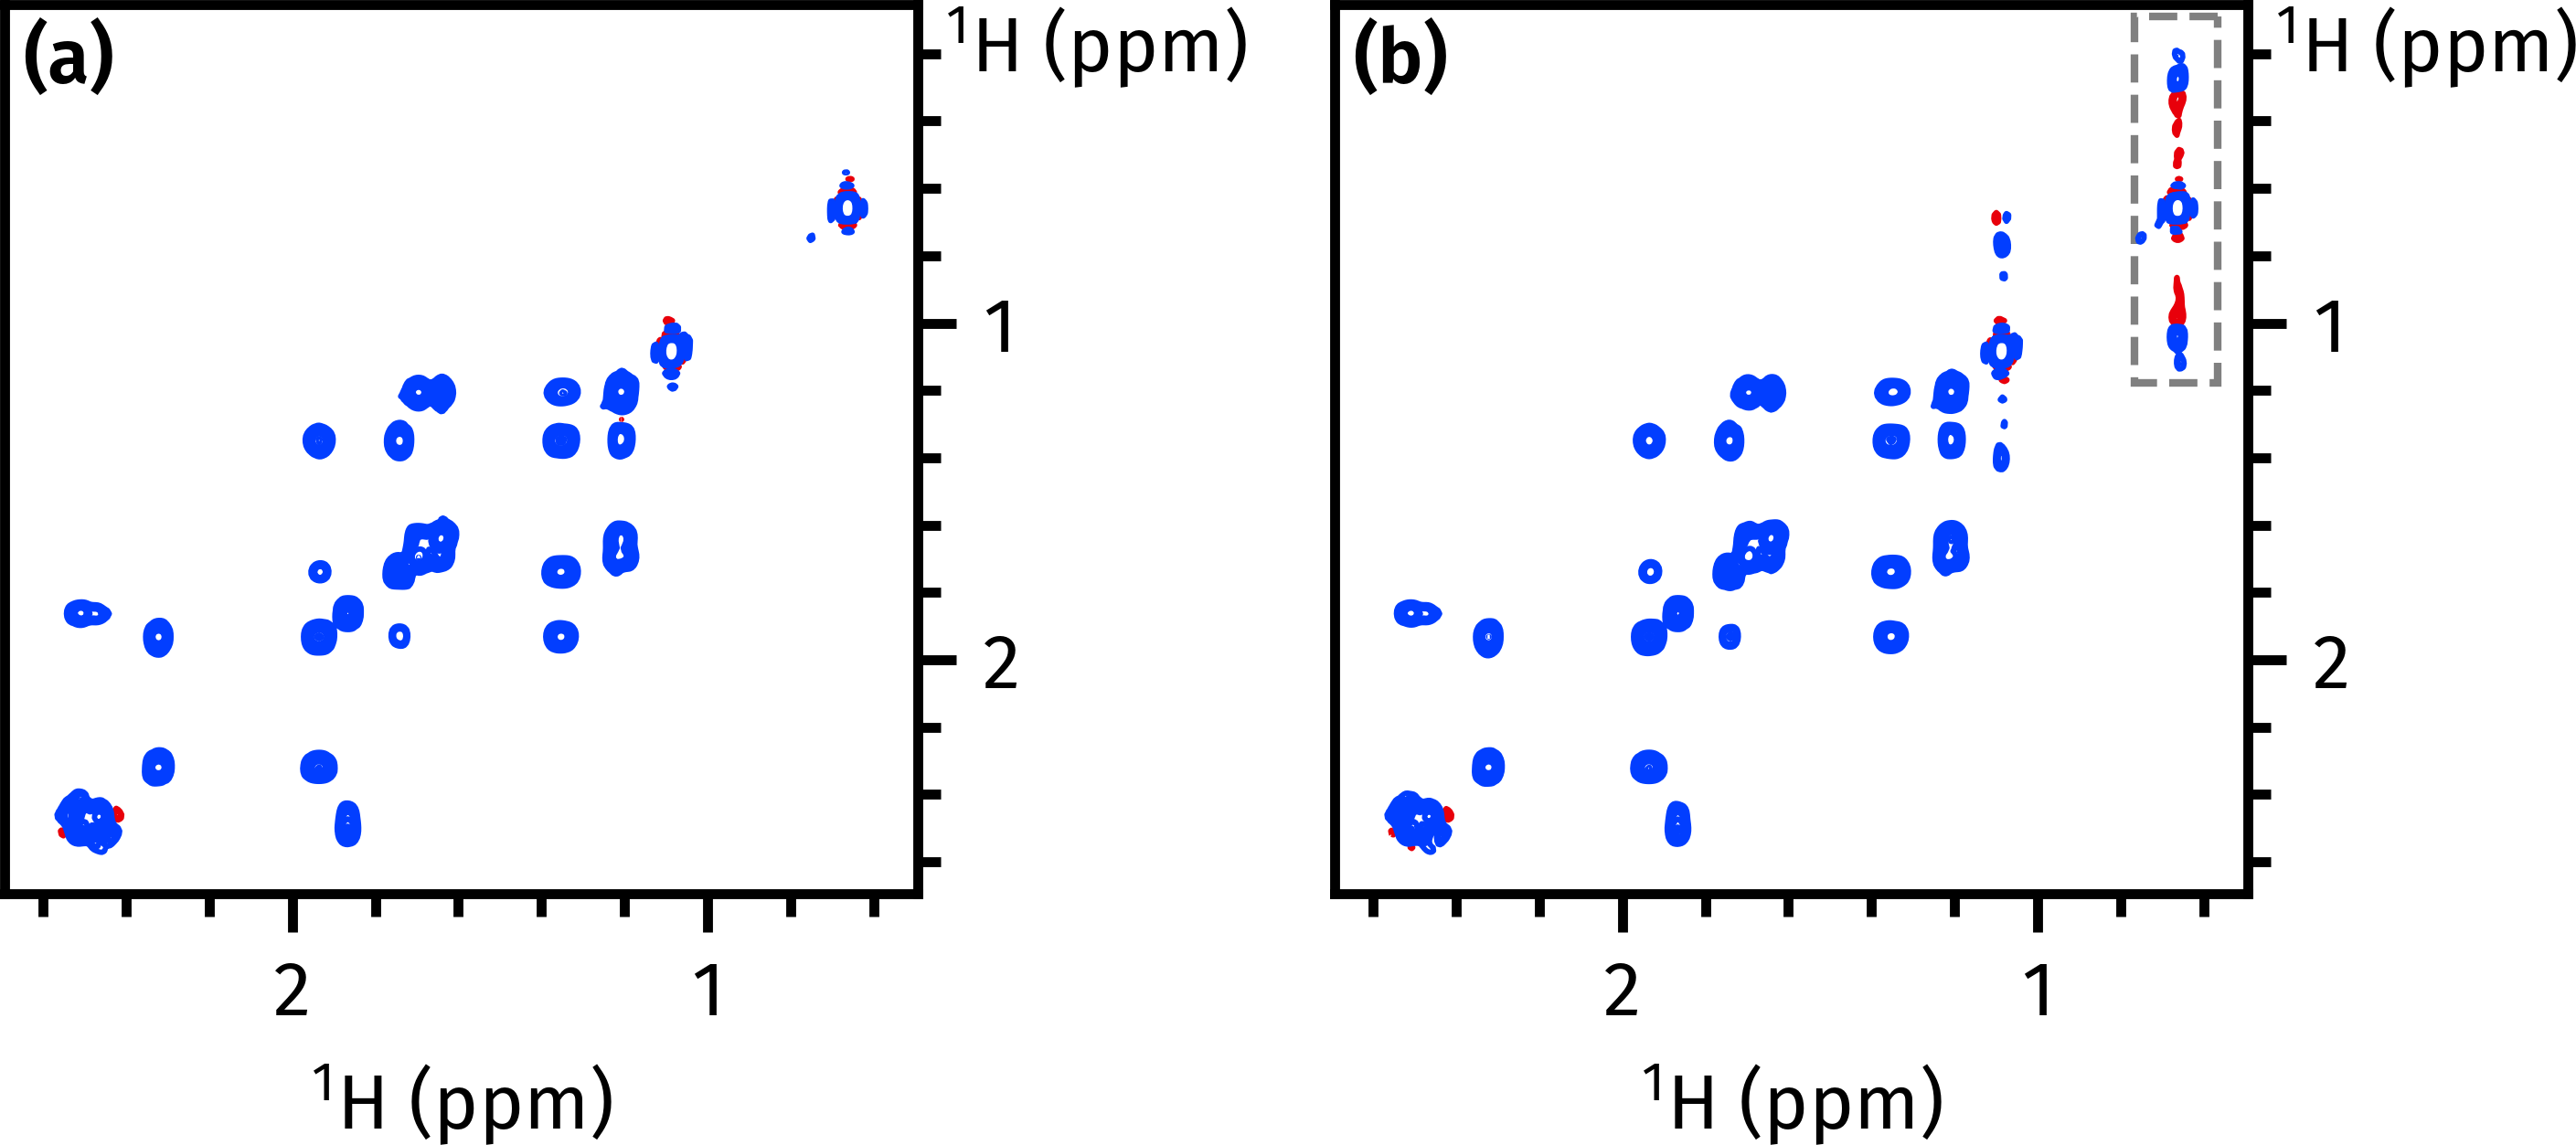
\includegraphics[draft=false]{noah/sehsqc_wing_arts.png}%
    {\phantomsubcaption\label{fig:sehsqc_wing_arts_2grad}}%
    {\phantomsubcaption\label{fig:sehsqc_wing_arts_1grad}}%
    \caption[Wing artefacts in CLIP-COSY spectra when extra seHSQC2 gradient is omitted]{
        Wing artefacts in CLIP-COSY spectra, taken from \noah{Sp,Cc} supersequences.
        \textbf{(\subref{fig:sehsqc_wing_arts_2grad})} Using the seHSQC2 module as shown in \cref{fig:sehsqc_po_noah2}.
        \textbf{(\subref{fig:sehsqc_wing_arts_1grad})} Using a modified seHSQC2 module where the gradient echo just before $t_1$ is removed.
        The wing artefacts flanking the two rightmost diagonal peaks can be clearly seen; the boxed artefacts are studied further in \cref{fig:sehsqc_wing_arts_proj}.
        \datacode{7A-201115}
    }
    \label{fig:sehsqc_wing_arts}
\end{figure}

A clue as to their origin is provided by the characteristic frequencies of the artefacts:
\begin{equation}
    \label{eq:wing_artefact_frequencies}
    \left(\Omega_1, \Omega_2 = \Omega_I \pm \frac{\Omega_I \cdot [t_{1,\text{HSQC}}/2]}{t_{1,\text{COSY}}}, \Omega_I\right)
\end{equation}
where $t_{1,\text{X}}$ refers to the value of $t_1$ in experiment X (it does not matter which increment is used, because the ratio of $t_1$ in the fraction above is constant).
In accordance with this, when the seHSQC indirect-dimension spectral width is reduced, the artefacts are displaced outwards (\cref{fig:sehsqc_wing_arts_proj_offon_sw4}).
This suggests that these artefacts arise from \magnnot{C} magnetisation which is frequency-labelled in two different $t_1$ periods: specifically, it evolves once during \textit{half} of the seHSQC $t_1$ period, and then again during the CLIP-COSY $t_1$ period.
In fact, it is necessary to apply CTP gradients on both sides of $t_1$ in order to suppress evolution of this stray magnetisation during both halves: if either or both of the gradients are removed, the artefacts are present (\cref{fig:sehsqc_wing_arts_proj_onon,fig:sehsqc_wing_arts_proj_offon,fig:sehsqc_wing_arts_proj_onoff,fig:sehsqc_wing_arts_proj_offoff}).

\begin{figure}[!ht]
    \centering
    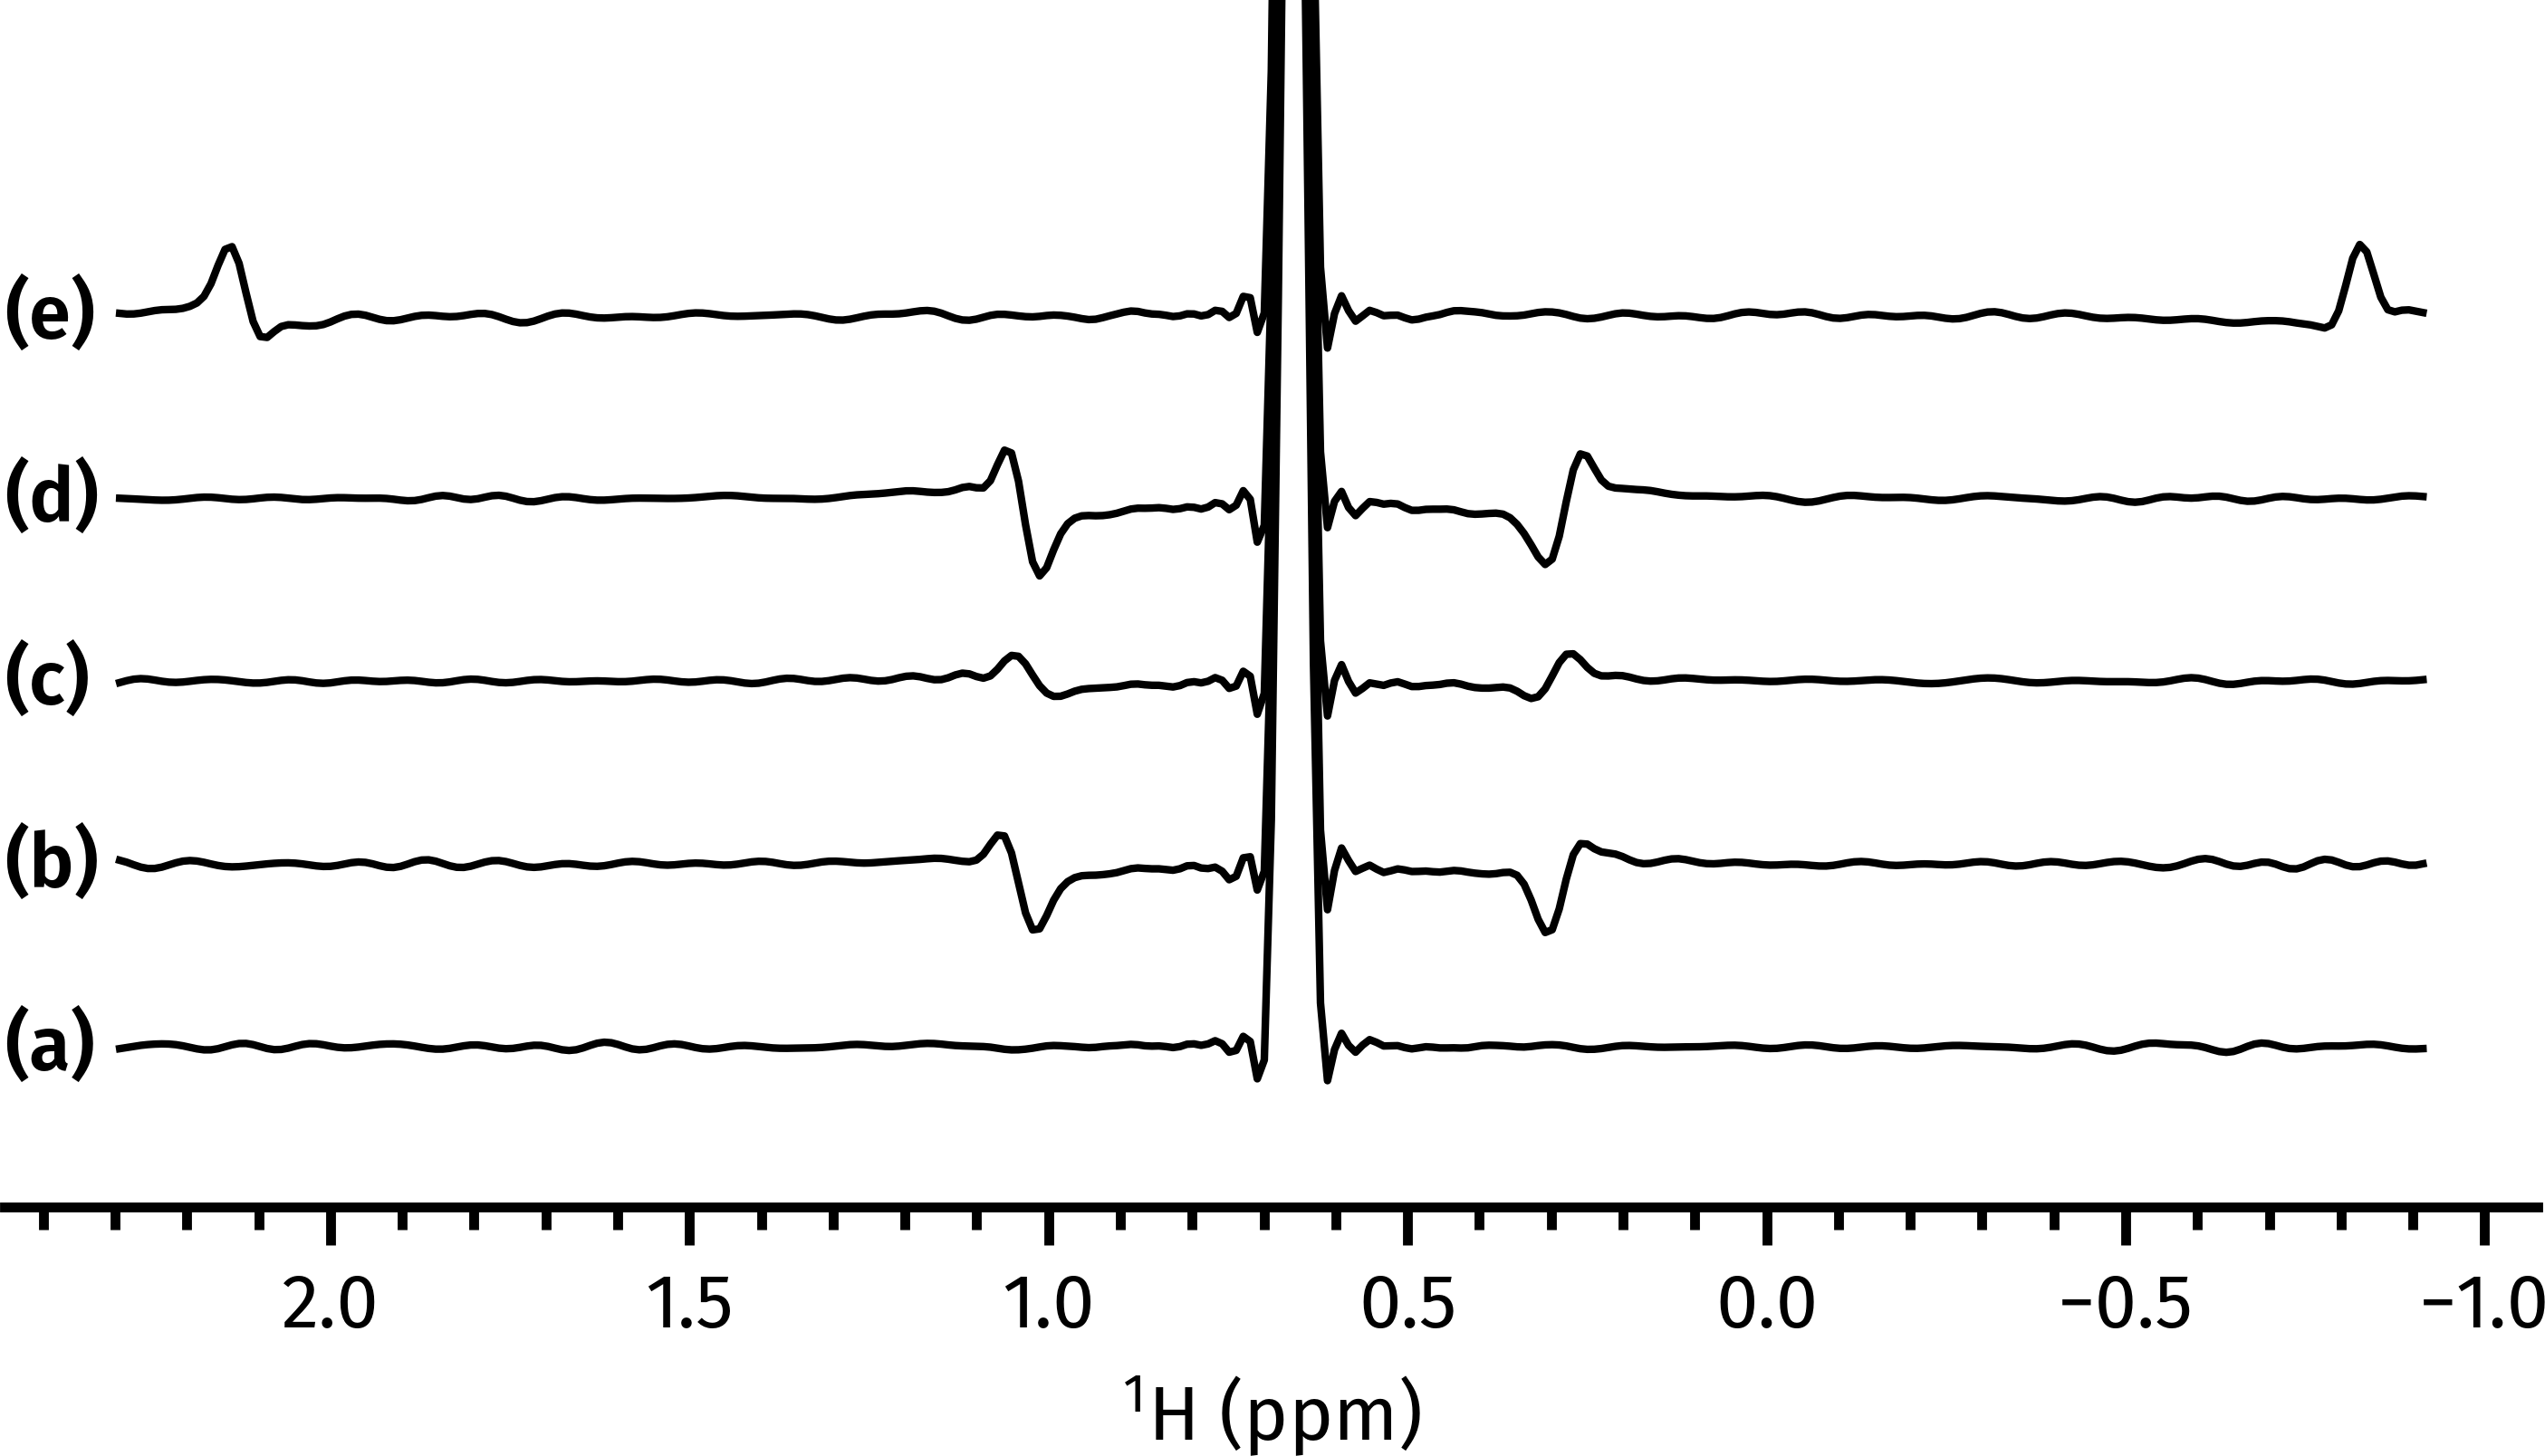
\includegraphics[draft=false]{noah/sehsqc_wing_arts_proj.png}%
    {\phantomsubcaption\label{fig:sehsqc_wing_arts_proj_onon}}%
    {\phantomsubcaption\label{fig:sehsqc_wing_arts_proj_offon}}%
    {\phantomsubcaption\label{fig:sehsqc_wing_arts_proj_onoff}}%
    {\phantomsubcaption\label{fig:sehsqc_wing_arts_proj_offoff}}%
    {\phantomsubcaption\label{fig:sehsqc_wing_arts_proj_offon_sw4}}%
    \caption[More detail about wing artefacts in CLIP-COSY spectra]{
        A closer look at wing artefacts in CLIP-COSY spectra, taken from \noah{Sp,Cc} supersequences with various modifications made to the seHSQC2 module.
        The spectra being plotted are 1D slices through $f_2 = \qty{0.67}{\ppm}$ of the 2D CLIP-COSY spectrum; this corresponds to the boxed region in \cref{fig:sehsqc_wing_arts_1grad}.
        \textbf{(\subref{fig:sehsqc_wing_arts_proj_onon})} Using the default seHSQC2 module, with one gradient before and one after $t_1$.
        \textbf{(\subref{fig:sehsqc_wing_arts_proj_offon})} The same as (\subref{fig:sehsqc_wing_arts_proj_onon}), but with the gradient before $t_1$ turned off (the spin echo is still present, but the gradient intensity is set to 0).
        \textbf{(\subref{fig:sehsqc_wing_arts_proj_onoff})} The same as (\subref{fig:sehsqc_wing_arts_proj_onon}), but with the gradient after $t_1$ turned off.
        \textbf{(\subref{fig:sehsqc_wing_arts_proj_offoff})} The same as (\subref{fig:sehsqc_wing_arts_proj_onon}), but with both gradients turned off.
        \textbf{(\subref{fig:sehsqc_wing_arts_proj_offon_sw4})} The same as (\subref{fig:sehsqc_wing_arts_proj_offon}), but with the seHSQC spectral width reduced by a factor of 4.
        \datacode{7A-201115}
    }
    \label{fig:sehsqc_wing_arts_proj}
\end{figure}

These wing artefacts are unique to fast-pulsing experiments such as NOAH supersequences: in a typical 2D experiment, these are less likely to arise because of the long(er) recovery delays between data acquisition periods.
In the sections which follow, we will see these surface repeatedly.
Fortunately, it proves to be relatively easy to suppress them through the judicious use of gradients.


\subsubsection{Multiplicity editing}

Multiplicity editing is reasonably easy to include in all of the seHSQC sequences above.
It suffices to add a spin echo of total duration $4\Delta = 1 / \oneJ{CH}$ just after $t_1$, while also making sure to change some pulse phases to account for the extra \proton{} \ang{180} pulse (\cref{fig:sehsqc_edited}).

\begin{figure}[!ht]
    \centering
    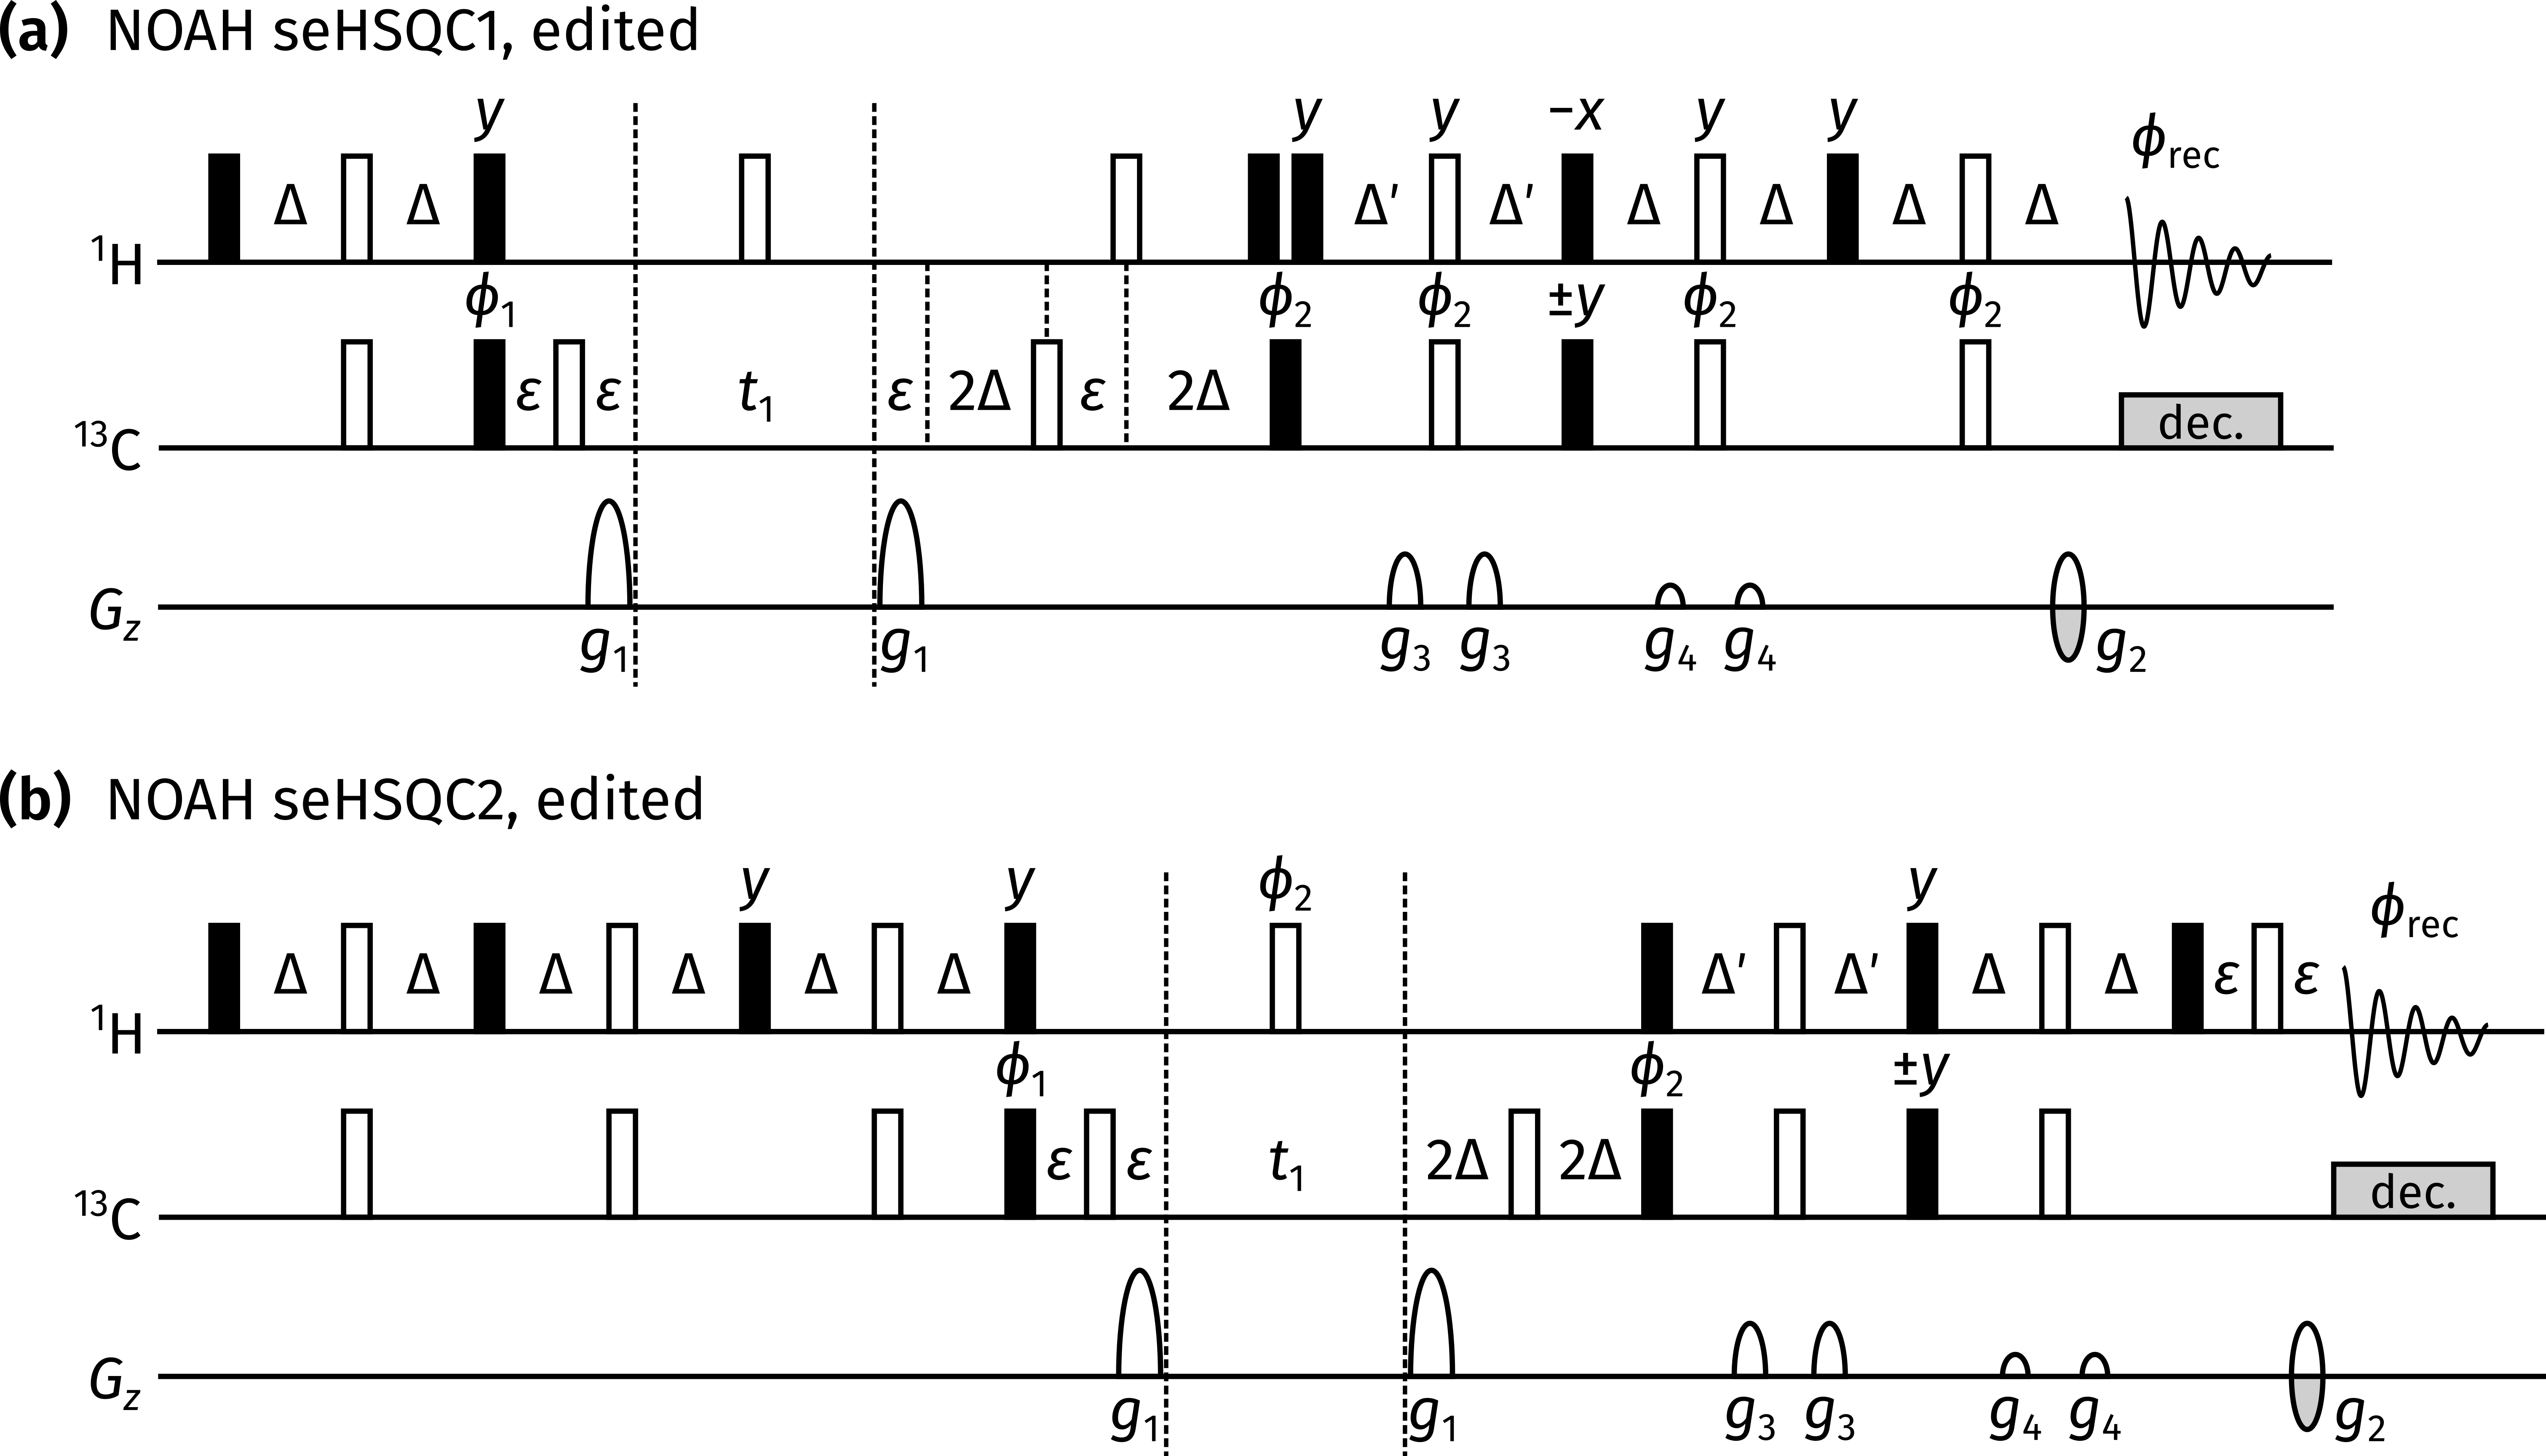
\includegraphics[draft=false]{pp/sehsqc/all_edited.png}%
    {\phantomsubcaption\label{fig:sehsqc_edited_1}}%
    {\phantomsubcaption\label{fig:sehsqc_edited_2}}%
    \caption[Multiplicity-edited NOAH seHSQC modules]{
        Multiplicity-edited NOAH seHSQC modules.
        \textbf{(\subref{fig:sehsqc_edited_1})} Edited seHSQC1.
        \textbf{(\subref{fig:sehsqc_edited_2})} Edited seHSQC2.
    }
    \label{fig:sehsqc_edited}
\end{figure}

\begin{figure}[!ht]
    \centering
    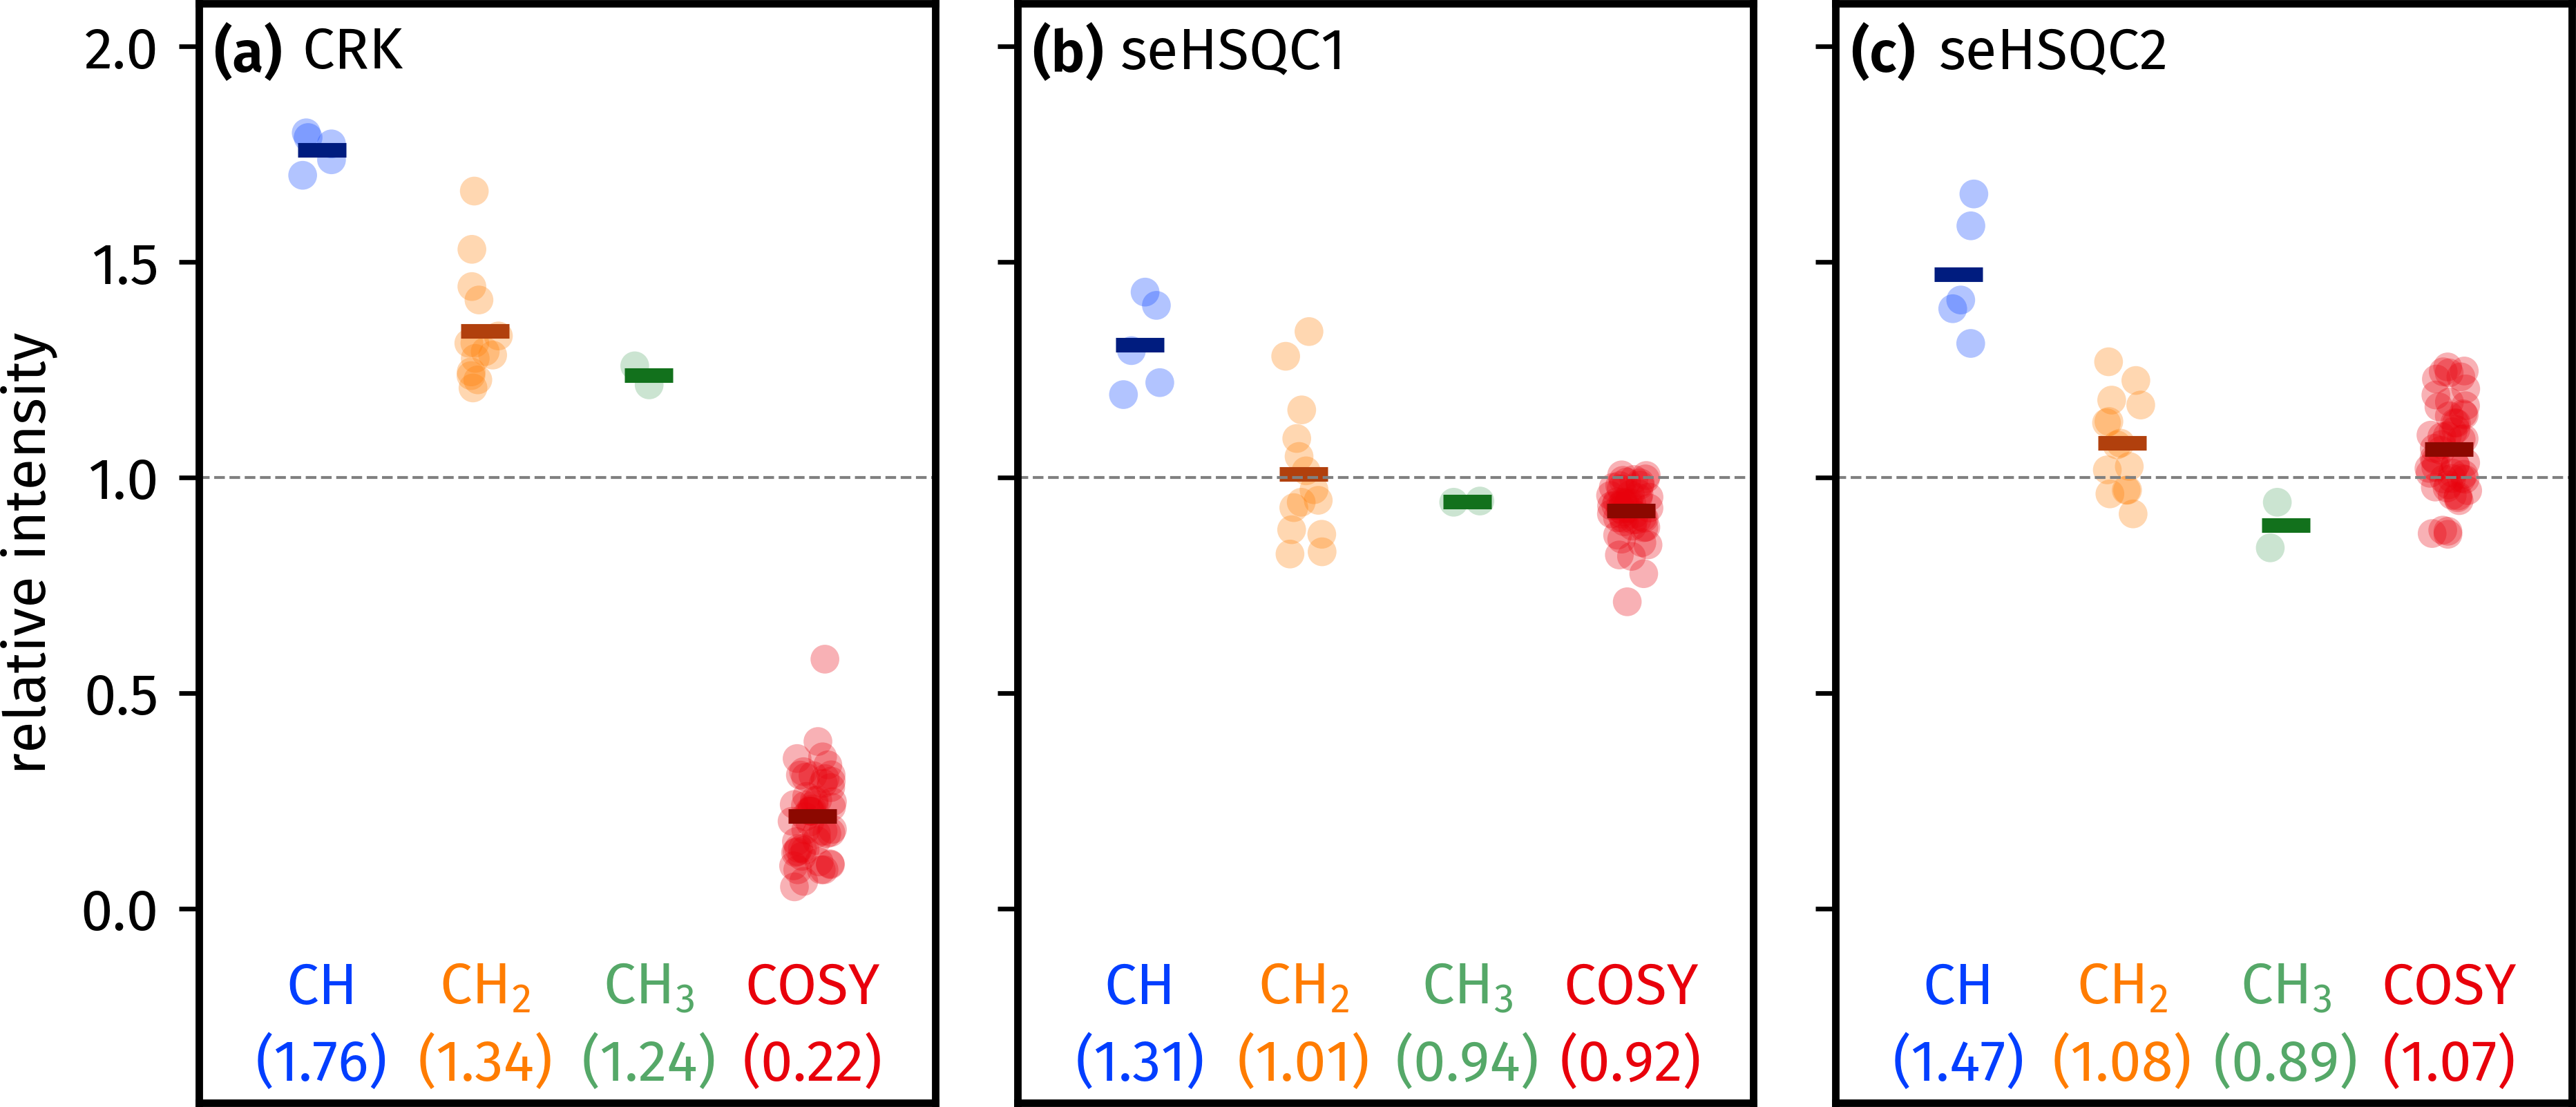
\includegraphics[draft=false]{noah/sehsqc_comp_edited.png}%
    {\phantomsubcaption\label{fig:noah_sehsqc_comp_edited_crk}}%
    {\phantomsubcaption\label{fig:noah_sehsqc_comp_edited_1}}%
    {\phantomsubcaption\label{fig:noah_sehsqc_comp_edited_2}}%
    \caption[Sensitivity comparisons for multiplicity-edited seHSQC]{
        Sensitivity comparisons for multiplicity-edited seHSQC in \noah{Sp,Cc} supersequences.
        The delay $\Delta'$ was set to $1 / (8 \cdot \oneJ{CH})$.
        \textbf{(\subref{fig:noah_sehsqc_comp_edited_crk})} Using the edited CRK seHSQC.
        \textbf{(\subref{fig:noah_sehsqc_comp_edited_1})} Using the edited seHSQC1 module.
        \textbf{(\subref{fig:noah_sehsqc_comp_edited_2})} Using the edited seHSQC2 module.
        \datacode{7A-201115}
    }
    \label{fig:noah_sehsqc_comp_edited}
\end{figure}

The inclusion of editing does not make a substantial difference in the sensitivity comparisons (\cref{fig:noah_sehsqc_comp_edited}).
However, it is interesting to note that the edited seHSQC2 in fact performs \textit{better} than the edited HSQC in terms of preserving bulk magnetisation, as evidenced by the larger COSY intensities in \cref{fig:noah_sehsqc_comp_edited_2}.
This can be explained by the fact that in the editing period of the HSQC experiment (and seHSQC1), the bulk magnetisation is placed in the transverse plane.
The evolution of homonuclear couplings will thus lead to a small loss in the amount of \magnnot{C} magnetisation preserved.
In the seHSQC2 sequence, the bulk magnetisation is longitudinal during the editing period, so does not evolve under $J_{\ch{HH}}$.


\subsubsection{Choice of $\symbf{\Delta'}$}

As discussed previously, there are several possible values for the delay $\Delta'$.
I thus also investigated the possibility of setting $\Delta' = 1 / (4 \cdot \oneJ{CH})$.
The corresponding sensitivity comparisons are shown in \cref{fig:noah_sehsqc_1over4j}.

\begin{figure}[!ht]
    \centering
    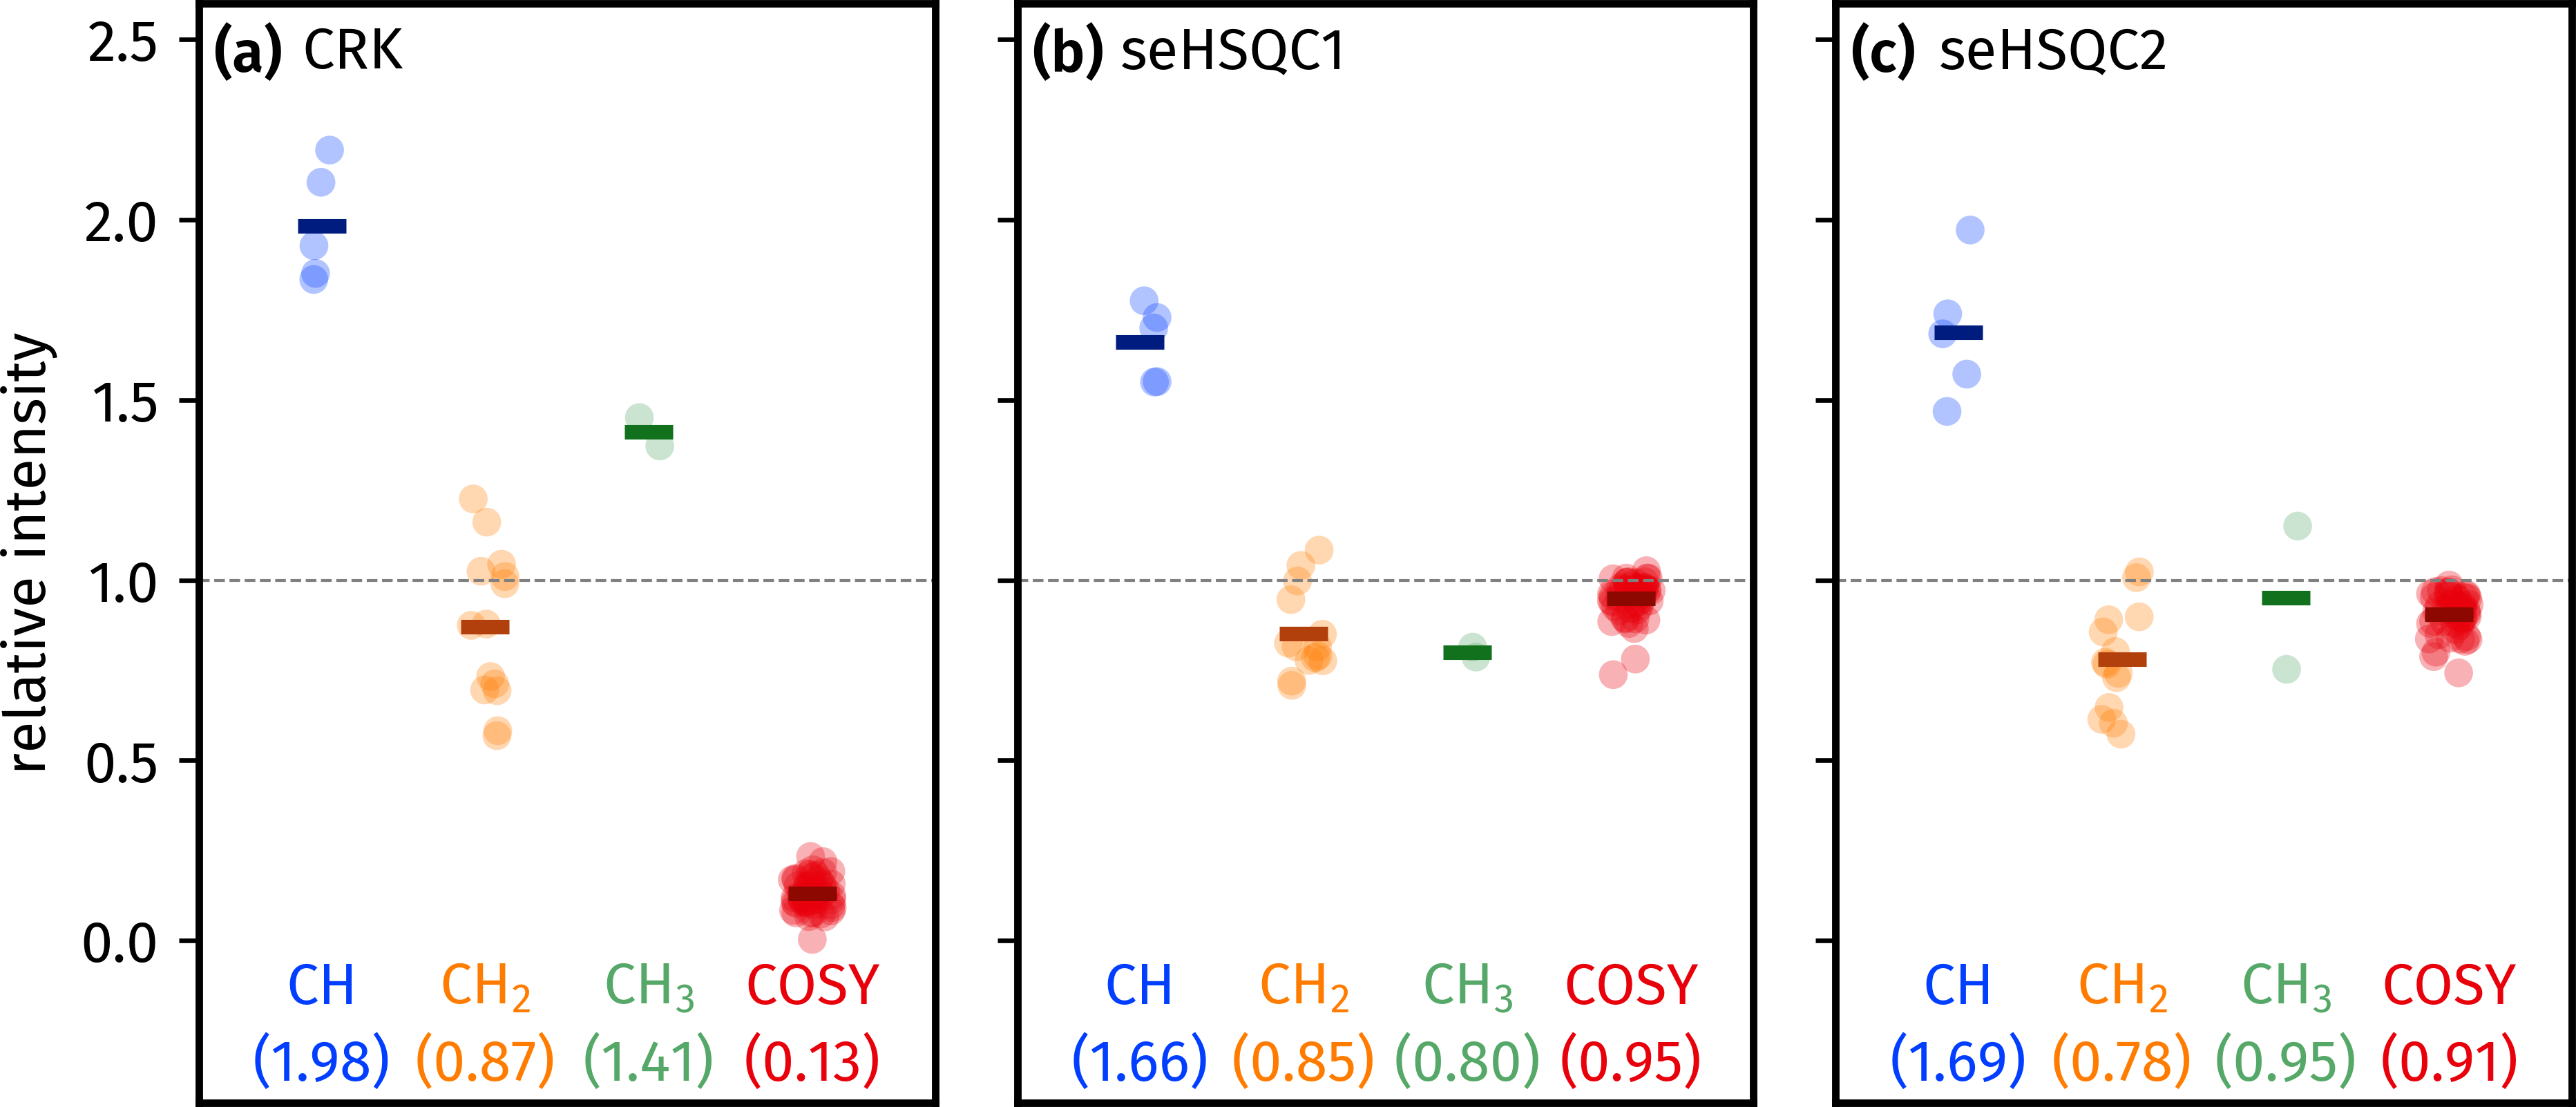
\includegraphics[draft=false]{noah/sehsqc_1over4j.png}%
    {\phantomsubcaption\label{fig:noah_sehsqc_1over4j_crk}}%
    {\phantomsubcaption\label{fig:noah_sehsqc_1over4j_1}}%
    {\phantomsubcaption\label{fig:noah_sehsqc_1over4j_2}}%
    \caption[Sensitivity comparisons for seHSQC with $\Delta' = 1 / (4 \cdot \oneJ{CH})$]{
        Sensitivity comparisons with $\Delta'$ set to $1 / (4 \cdot \oneJ{CH})$.
        Multiplicity editing was not used.
        \textbf{(\subref{fig:noah_sehsqc_1over4j_crk})} Using the edited CRK seHSQC.
        \textbf{(\subref{fig:noah_sehsqc_1over4j_1})} Using the edited seHSQC1 module.
        \textbf{(\subref{fig:noah_sehsqc_1over4j_2})} Using the edited seHSQC2 module.
        \datacode{7A-201115}
    }
    \label{fig:noah_sehsqc_1over4j}
\end{figure}

As can be appreciated, the sensitivity boosts obtained for \ch{CH} groups is higher than in the corresponding spectra with $\Delta' = 1 / (8 \cdot \oneJ{CH}$ (\cref{fig:noah_sehsqc_comp}).
However, in this case, there is a small sensitivity \textit{loss} for \ch{CH2} and \ch{CH3} groups as compared to the original HSQC (which is consistent with previous studies\autocite{Schleucher1994JBNMR}).
For \ch{CH3} groups this is unlikely to be of any consequence, but particularly for diastereotopic \ch{CH2} groups this may not be desirable.

The conclusions are entirely similar when multiplicity editing is enabled (\cref{fig:noah_sehsqc_1over4j_edited}), so will not be further discussed.

\begin{figure}[!ht]
    \centering
    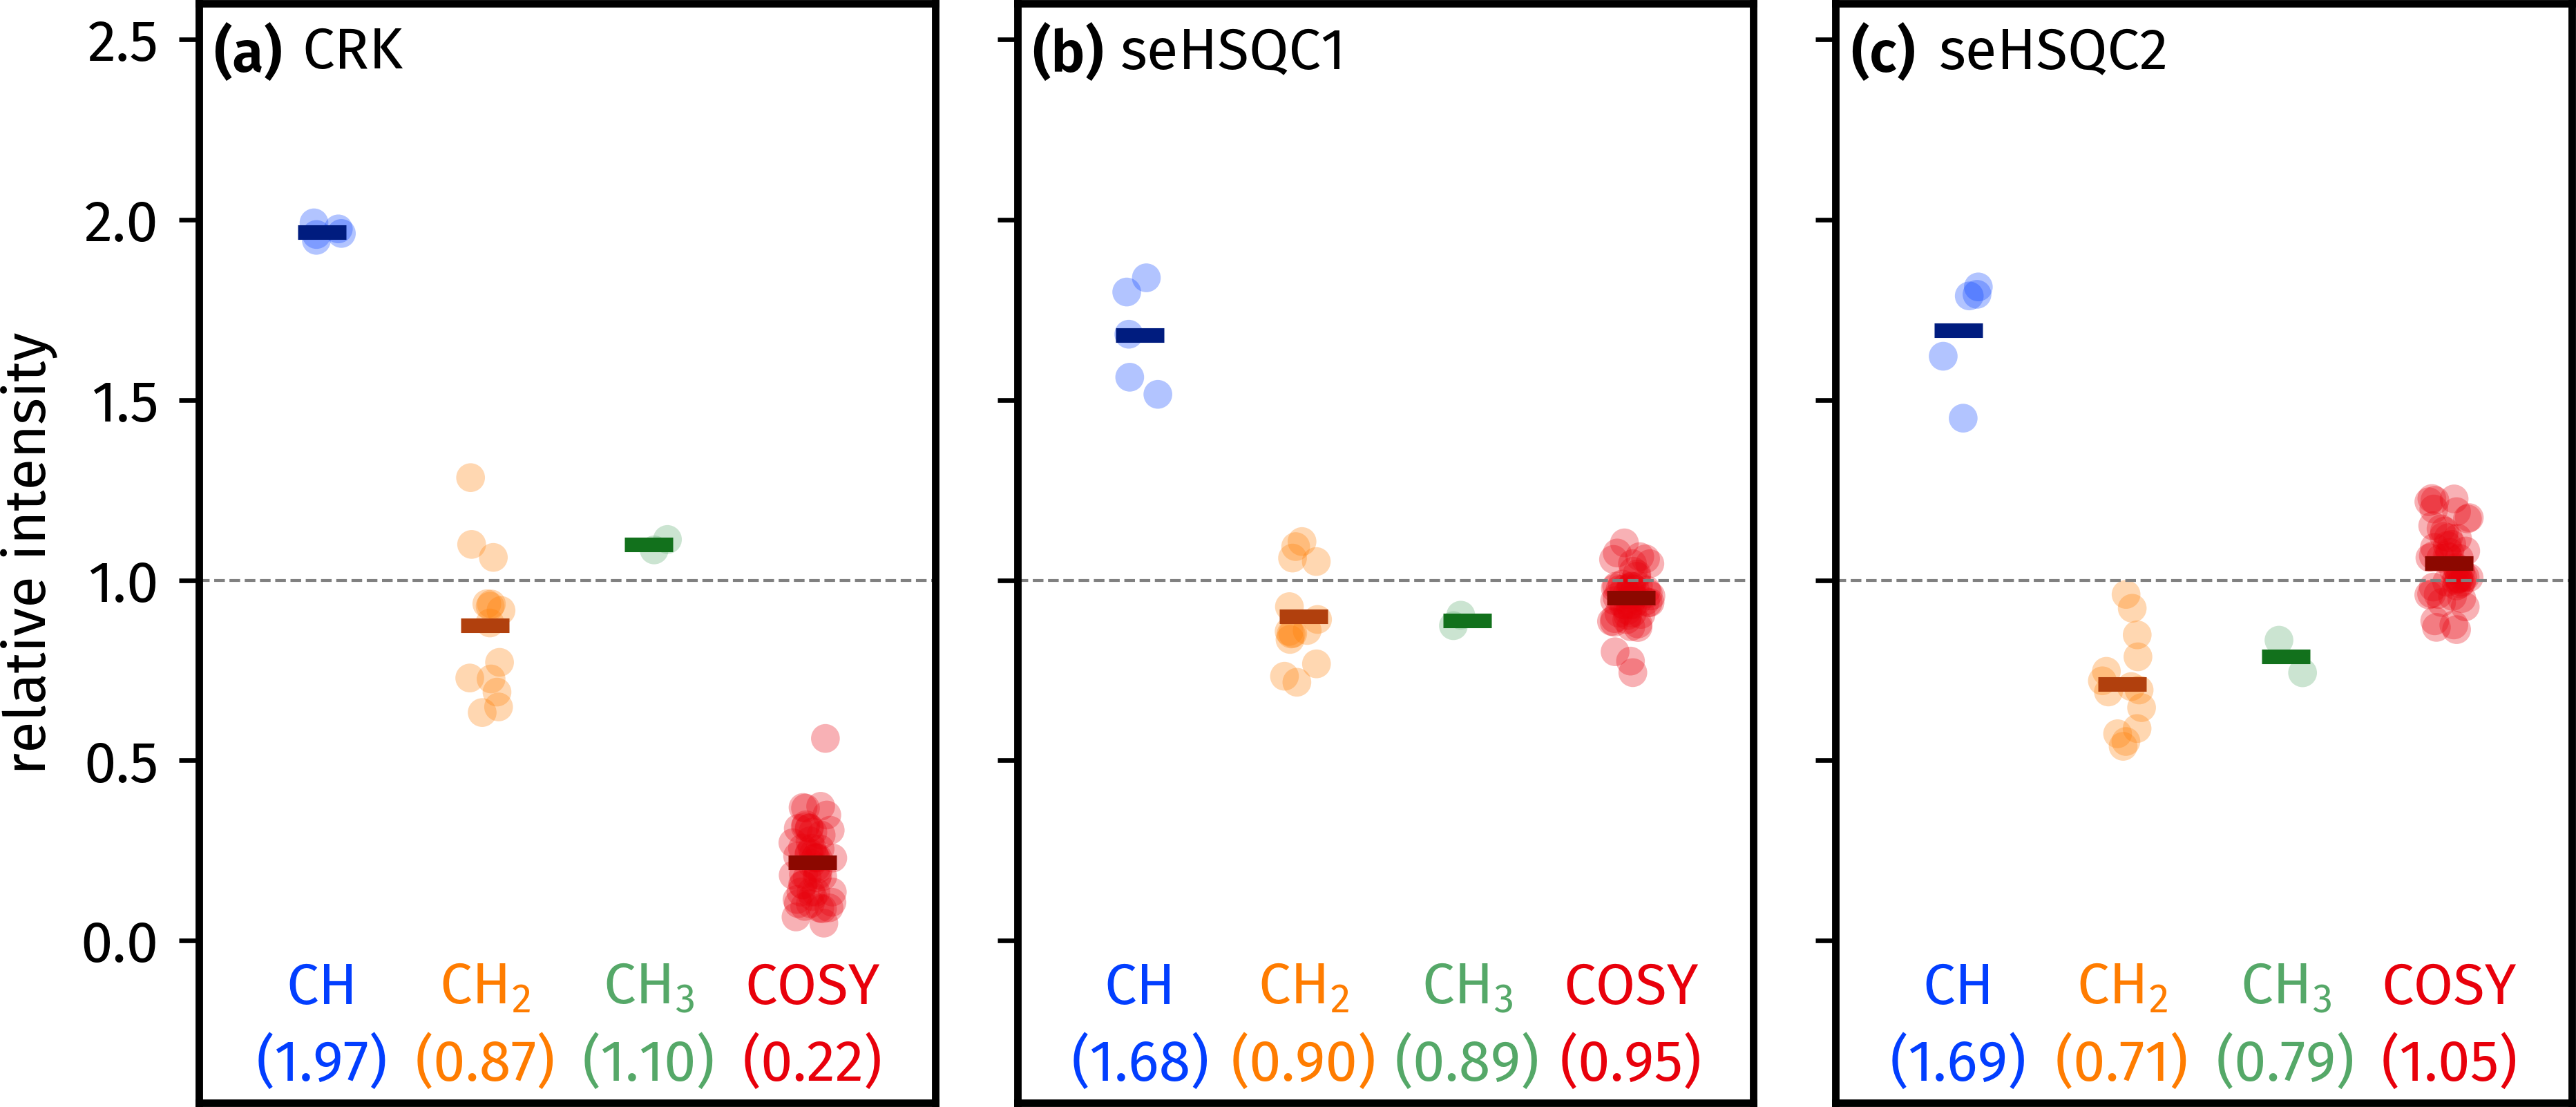
\includegraphics[draft=false]{noah/sehsqc_1over4j_edited.png}%
    {\phantomsubcaption\label{fig:noah_sehsqc_1over4j_edited_crk}}%
    {\phantomsubcaption\label{fig:noah_sehsqc_1over4j_edited_1}}%
    {\phantomsubcaption\label{fig:noah_sehsqc_1over4j_edited_2}}%
    \caption[Sensitivity comparisons for edited seHSQC with $\Delta' = 1 / (4 \cdot \oneJ{CH})$]{
        Sensitivity comparisons with $\Delta'$ set to $1 / (4 \cdot \oneJ{CH})$ and with multiplicity editing.
        \textbf{(\subref{fig:noah_sehsqc_1over4j_edited_crk})} Using the edited CRK seHSQC.
        \textbf{(\subref{fig:noah_sehsqc_1over4j_edited_1})} Using the edited seHSQC1 module.
        \textbf{(\subref{fig:noah_sehsqc_1over4j_edited_2})} Using the edited seHSQC2 module.
        \datacode{7A-201115}
    }
    \label{fig:noah_sehsqc_1over4j_edited}
\end{figure}




\subsubsection{Optimal control for seHSQC1}

One unresolved question is why the seHSQC1 module has a lower sensitivity than the seHSQC2, despite being shorter and containing fewer \ang{180} pulses.
There is also nothing in the product operator analysis to explain why this should be the case.
One remaining possibility is the presence of some non-ideality in the pulses themselves, and the composite \proton{} pulse is an obvious candidate for investigation.%
\footnote{The concept of a \textit{composite pulse}\autocite{Levitt1986PNMRS} is usually associated with greater efficiency / uniformity, but here I have used the term to loosely refer to a consecutive series of pulses.}

In order to investigate the extent to which this was responsible, I sought to use optimal control theory to develop a \textit{universal rotation pulse} (URP) which could replace this composite pulse.
Such a pulse must accomplish the transformations in \cref{eq:sehsqc1_dp}, namely $z \to y$ and $y \to x$.%
\footnote{The effect of this pulse on $x$-magnetisation is not important for the seHSQC1, but is in fact fully determined by these two constraints: $UI_x\adj{U} = -\mi U(I_yI_z - I_zI_y)\adj{U} = -\mi(UI_y\adj{U}UI_z\adj{U} - UI_z\adj{U}UI_y\adj{U}) = -\mi(I_xI_y - I_yI_x) = I_z$.
This reveals a geometric interpretation of this pulse element: it is actually a \ang{120} rotation about the vector $(1, 1, 1)$, which is closely related to the $C_3$ symmetry operation in the octahedral point group.}
This optimisation was performed using an interior-point algorithm (the default in Matlab \texttt{fmincon}) and the ESCALADE method\autocite{Foroozandeh2021A} for the calculation of analytic derivatives.
Pulse fidelity was calculated as an average over 51 \proton{} spins, evenly distributed across a frequency range of \qty{11}{kHz} (corresponding to \qty{15.7}{\ppm} at \qty{700}{\MHz}); the duration of the pulse was fixed at \qty{200}{\us}, and 200 pulse points were used.

The \carbon{} \ang{90} pulse which is simultaneously applied during the pulse sequence was not optimised together with this: because of the longer duration of the \proton{} URP, the sequence must be modified slightly (\cref{fig:sehsqc1_urp}).
In particular, the delays $\alpha$ and $\beta$ must be chosen in order to satisfy the relations $2\varepsilon = \alpha + \beta$ (to ensure \magnnot{C} magnetisation is refocused), and $\alpha = \beta + \tau$ (to ensure that for \magn{C} magnetisation, the \carbon{} chemical shift evolves for a total duration of $t_1$).

\begin{figure}[!ht]
    \centering
    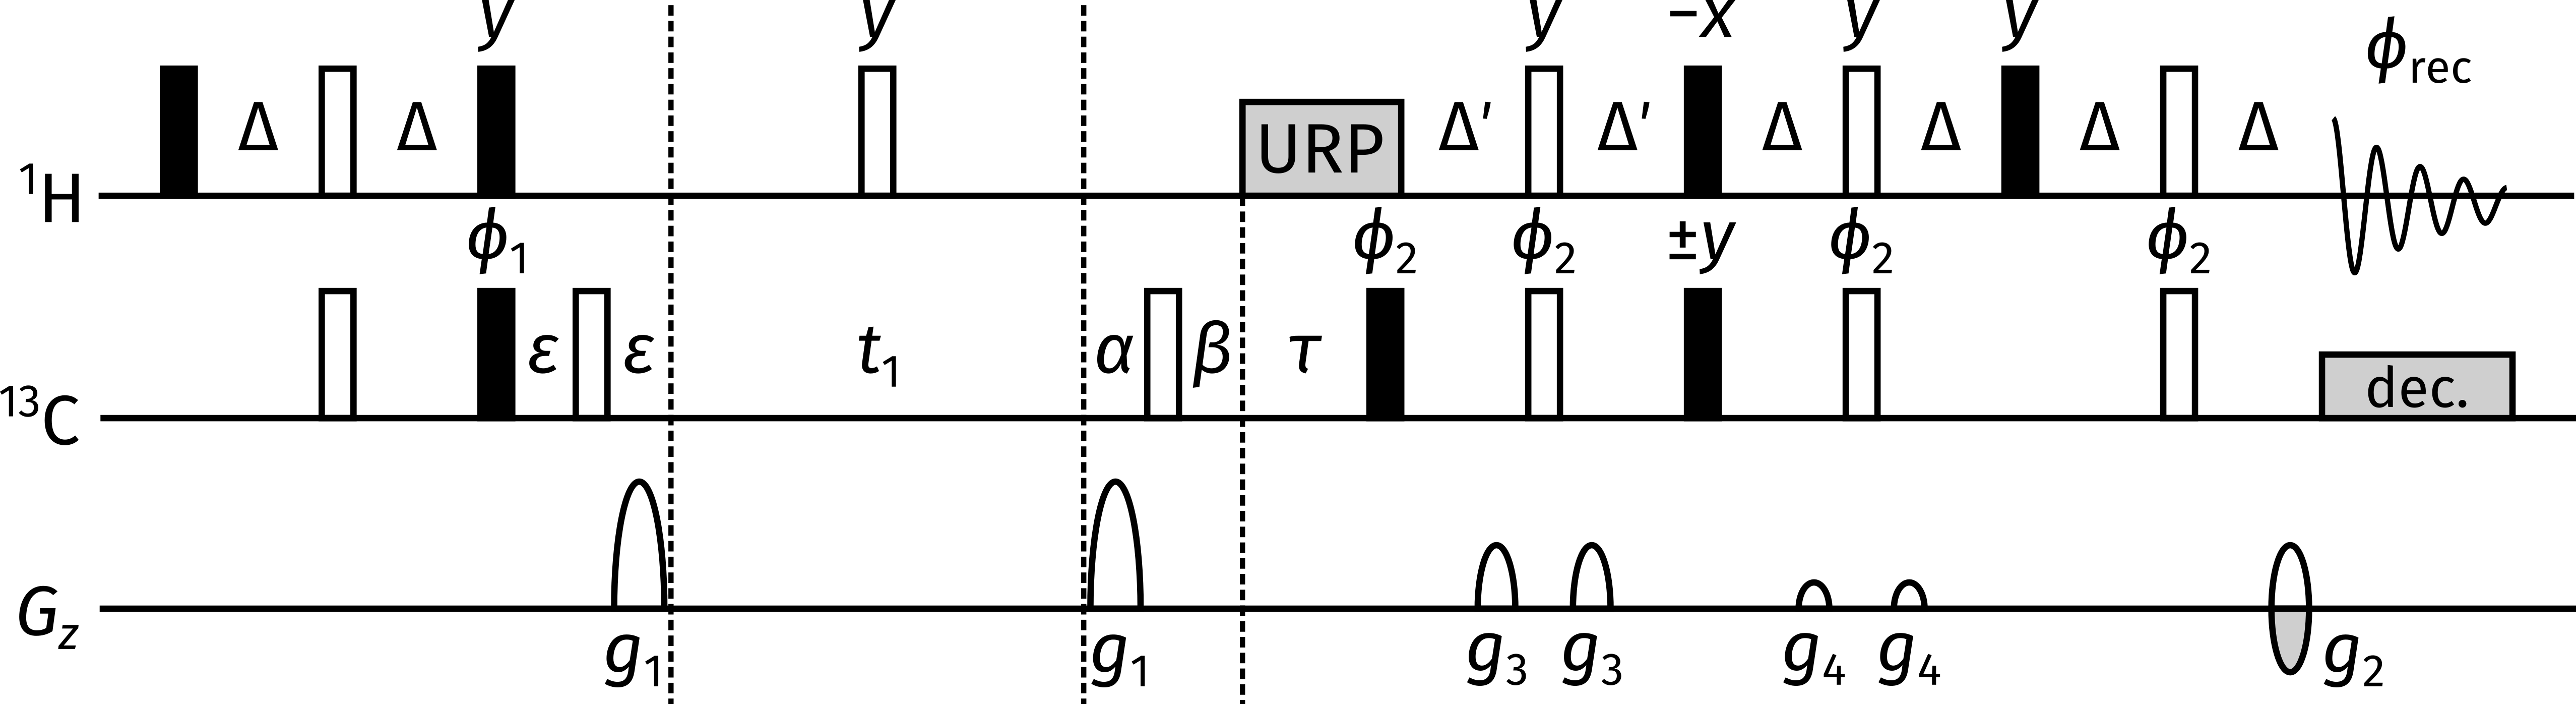
\includegraphics[draft=false]{pp/sehsqc/1urp.png}%
    \caption[seHSQC1 pulse sequence with \proton{} URP]{
        seHSQC1 pulse sequence using a \proton{} URP in place of the double-\ang{90} composite pulse.
        $\tau$ is the difference in duration between the URP and the \carbon{} \ang{90} hard pulse.
        Delays are set as: $\alpha = \varepsilon + \tau/2$; $\beta = \varepsilon - \tau/2$.
    }
    \label{fig:sehsqc1_urp}
\end{figure}

\begin{figure}[!ht]
    \centering
    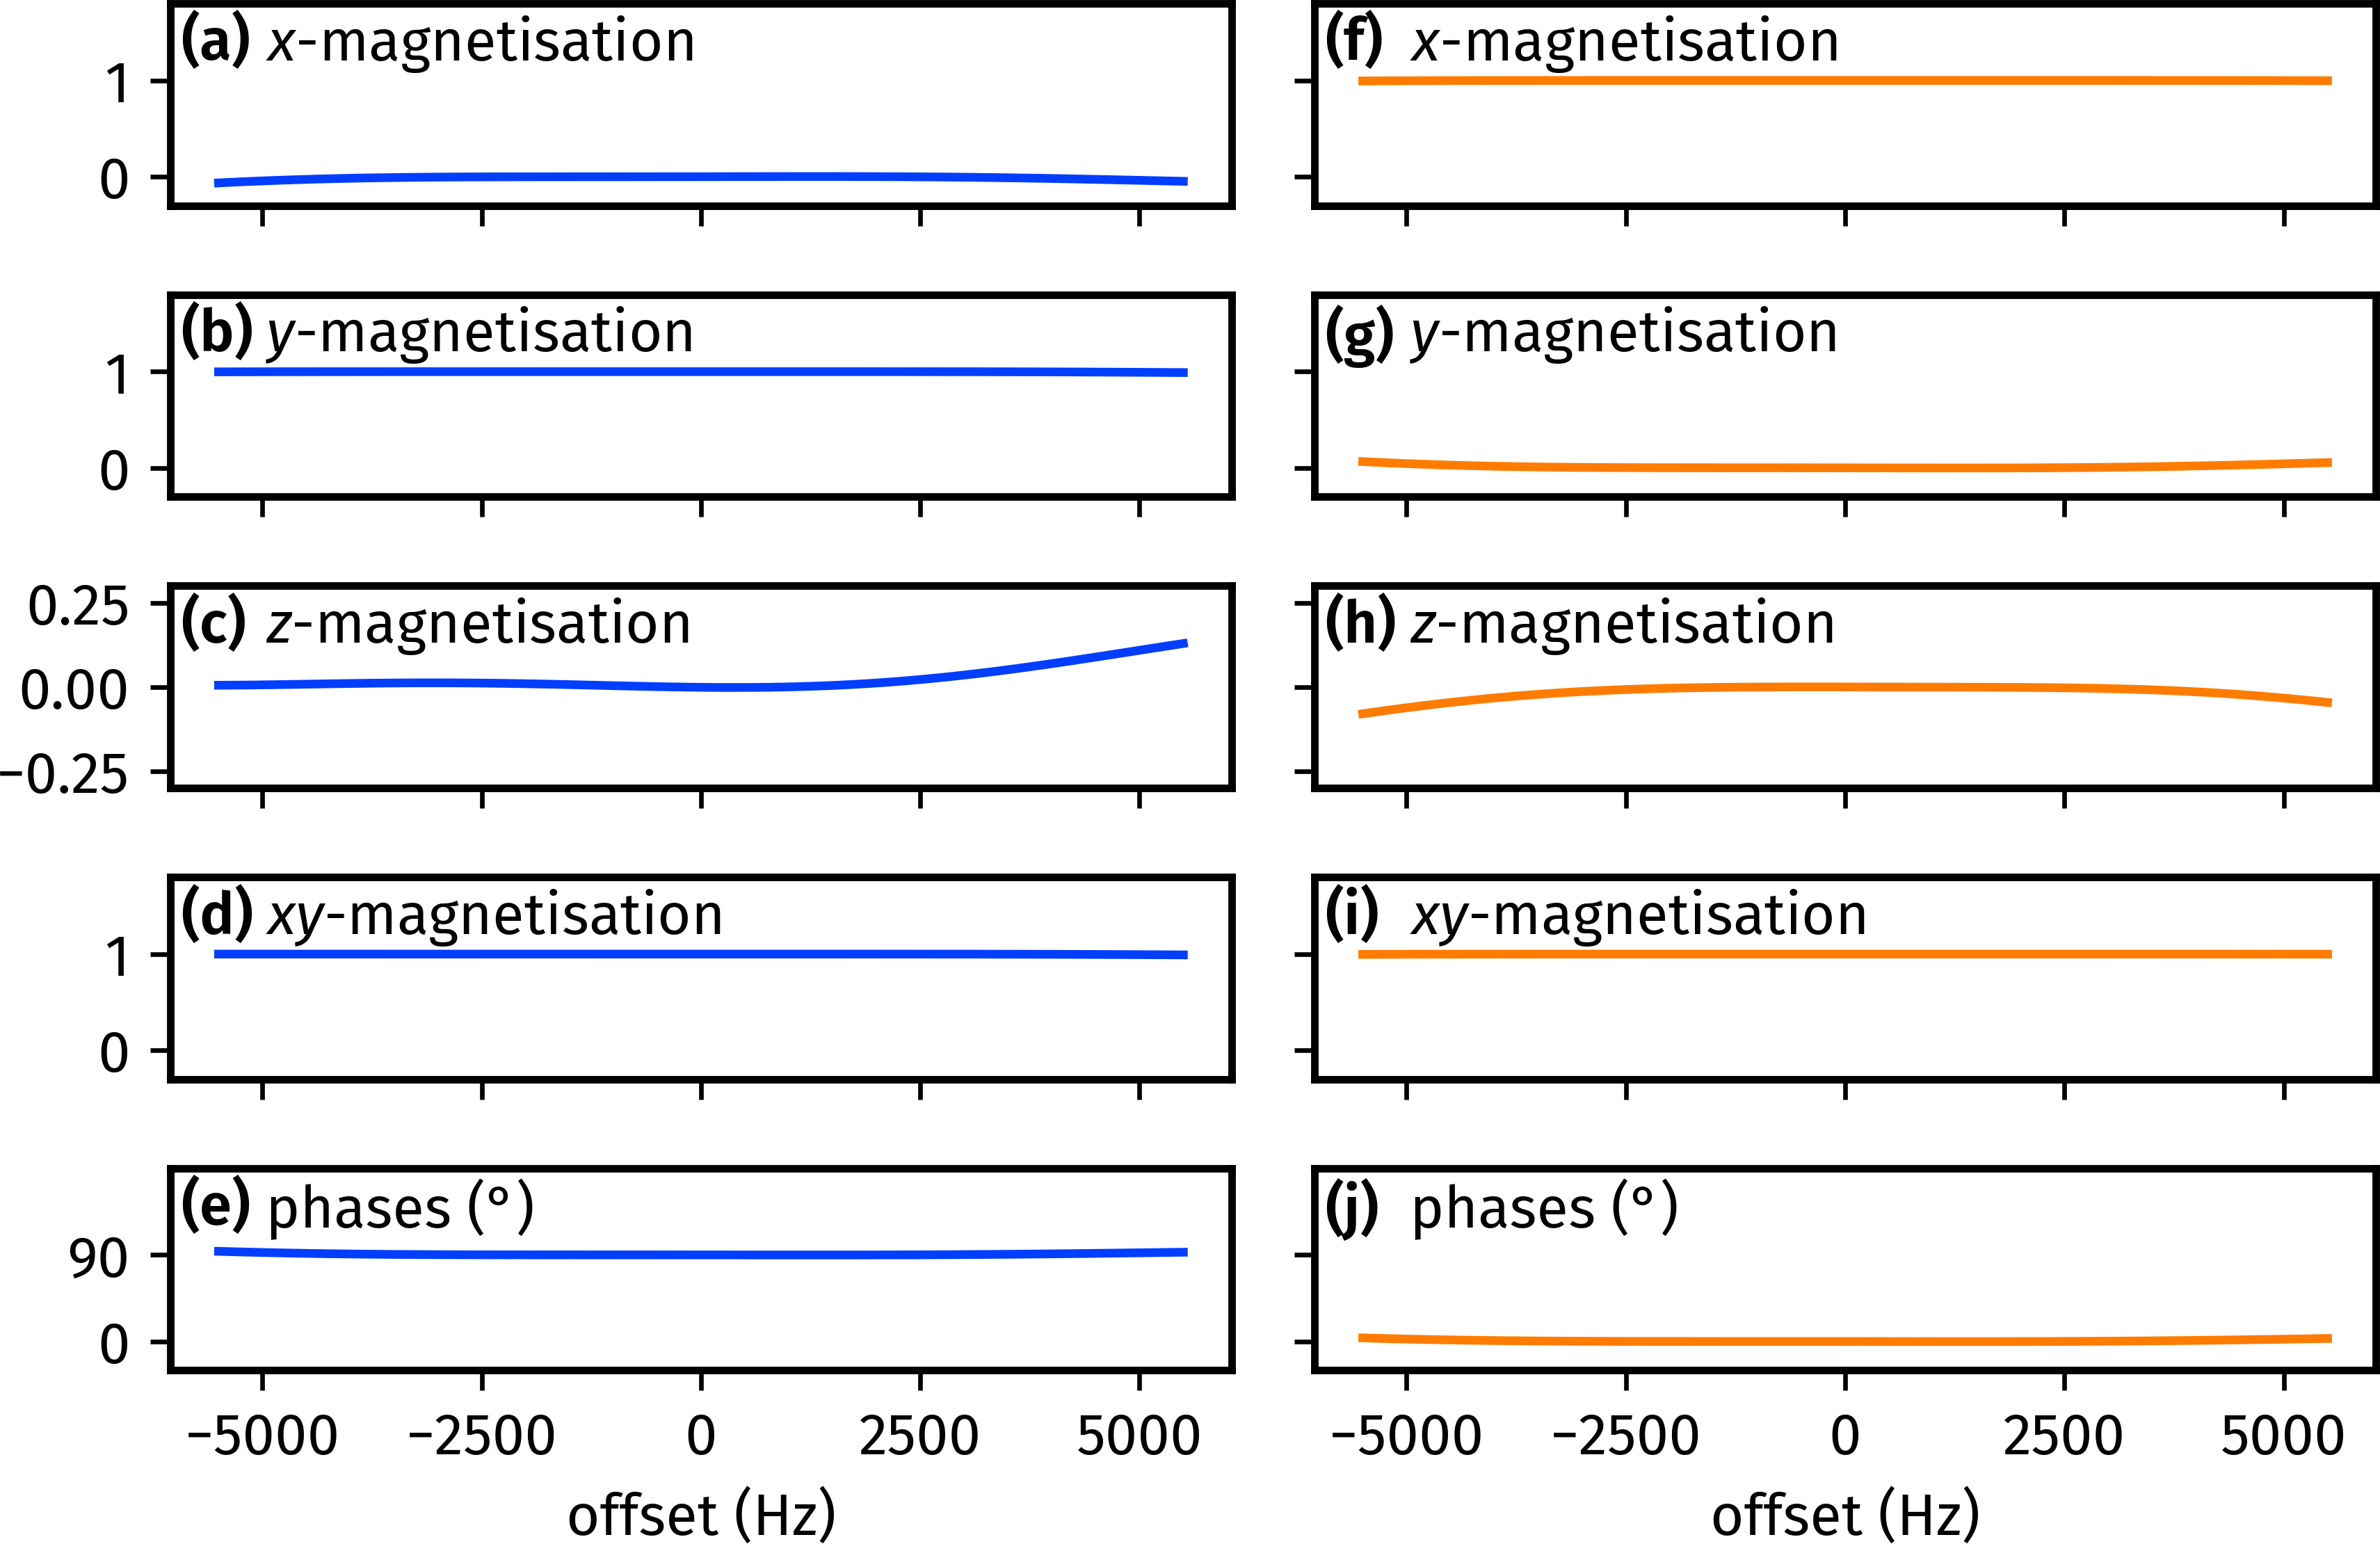
\includegraphics[draft=false]{noah/spv1_urp_magn.png}%
    {\phantomsubcaption\label{fig:spv1_urp_magn_z_x}}%
    {\phantomsubcaption\label{fig:spv1_urp_magn_z_y}}%
    {\phantomsubcaption\label{fig:spv1_urp_magn_z_z}}%
    {\phantomsubcaption\label{fig:spv1_urp_magn_z_xy}}%
    {\phantomsubcaption\label{fig:spv1_urp_magn_z_phase}}%
    {\phantomsubcaption\label{fig:spv1_urp_magn_y_x}}%
    {\phantomsubcaption\label{fig:spv1_urp_magn_y_y}}%
    {\phantomsubcaption\label{fig:spv1_urp_magn_y_z}}%
    {\phantomsubcaption\label{fig:spv1_urp_magn_y_xy}}%
    {\phantomsubcaption\label{fig:spv1_urp_magn_y_phase}}%
    \caption[Simulated performance of URP used for seHSQC1 module]{
        Simulated performance of URP used for seHSQC1 module on $z$- and $y$-magnetisation. The pulse fidelity was 99.99\%.
        \textbf{(\subref{fig:spv1_urp_magn_z_x})--(\subref{fig:spv1_urp_magn_z_phase})} Using $z$-magnetisation as input: the plots respectively show the amount of $x$-magnetisation, $y$-magnetisation, $z$-magnetisation, transverse magnetisation ($M_{xy} = \sqrt{M_x^2 + M_y^2}$), and the phase of the transverse magnetisation generated, as a function of offset frequency.
        \textbf{(\subref{fig:spv1_urp_magn_y_x})--(\subref{fig:spv1_urp_magn_y_phase})} The same, but using $y$-magnetisation as input.
    }
    \label{fig:spv1_urp_magn}
\end{figure}

This optimisation process yielded a pulse with 99.99\% fidelity: the (theoretical) performance of this pulse on $z$- and $y$-magnetisation is shown in \cref{fig:spv1_urp_magn}.
However, when tested in the actual seHSQC1 experiment, this failed to yield any substantial difference compared to the original double \ang{90} pulse (\cref{fig:sehsqc1_urp_sens_1dp,fig:sehsqc1_urp_sens_1urp}).
Importantly, the performance still falls below that of the seHSQC2 module (\cref{fig:sehsqc1_urp_sens_2}).
The reason for the poorer sensitivity therefore likely lies elsewhere.

\begin{figure}[htb]
    \centering
    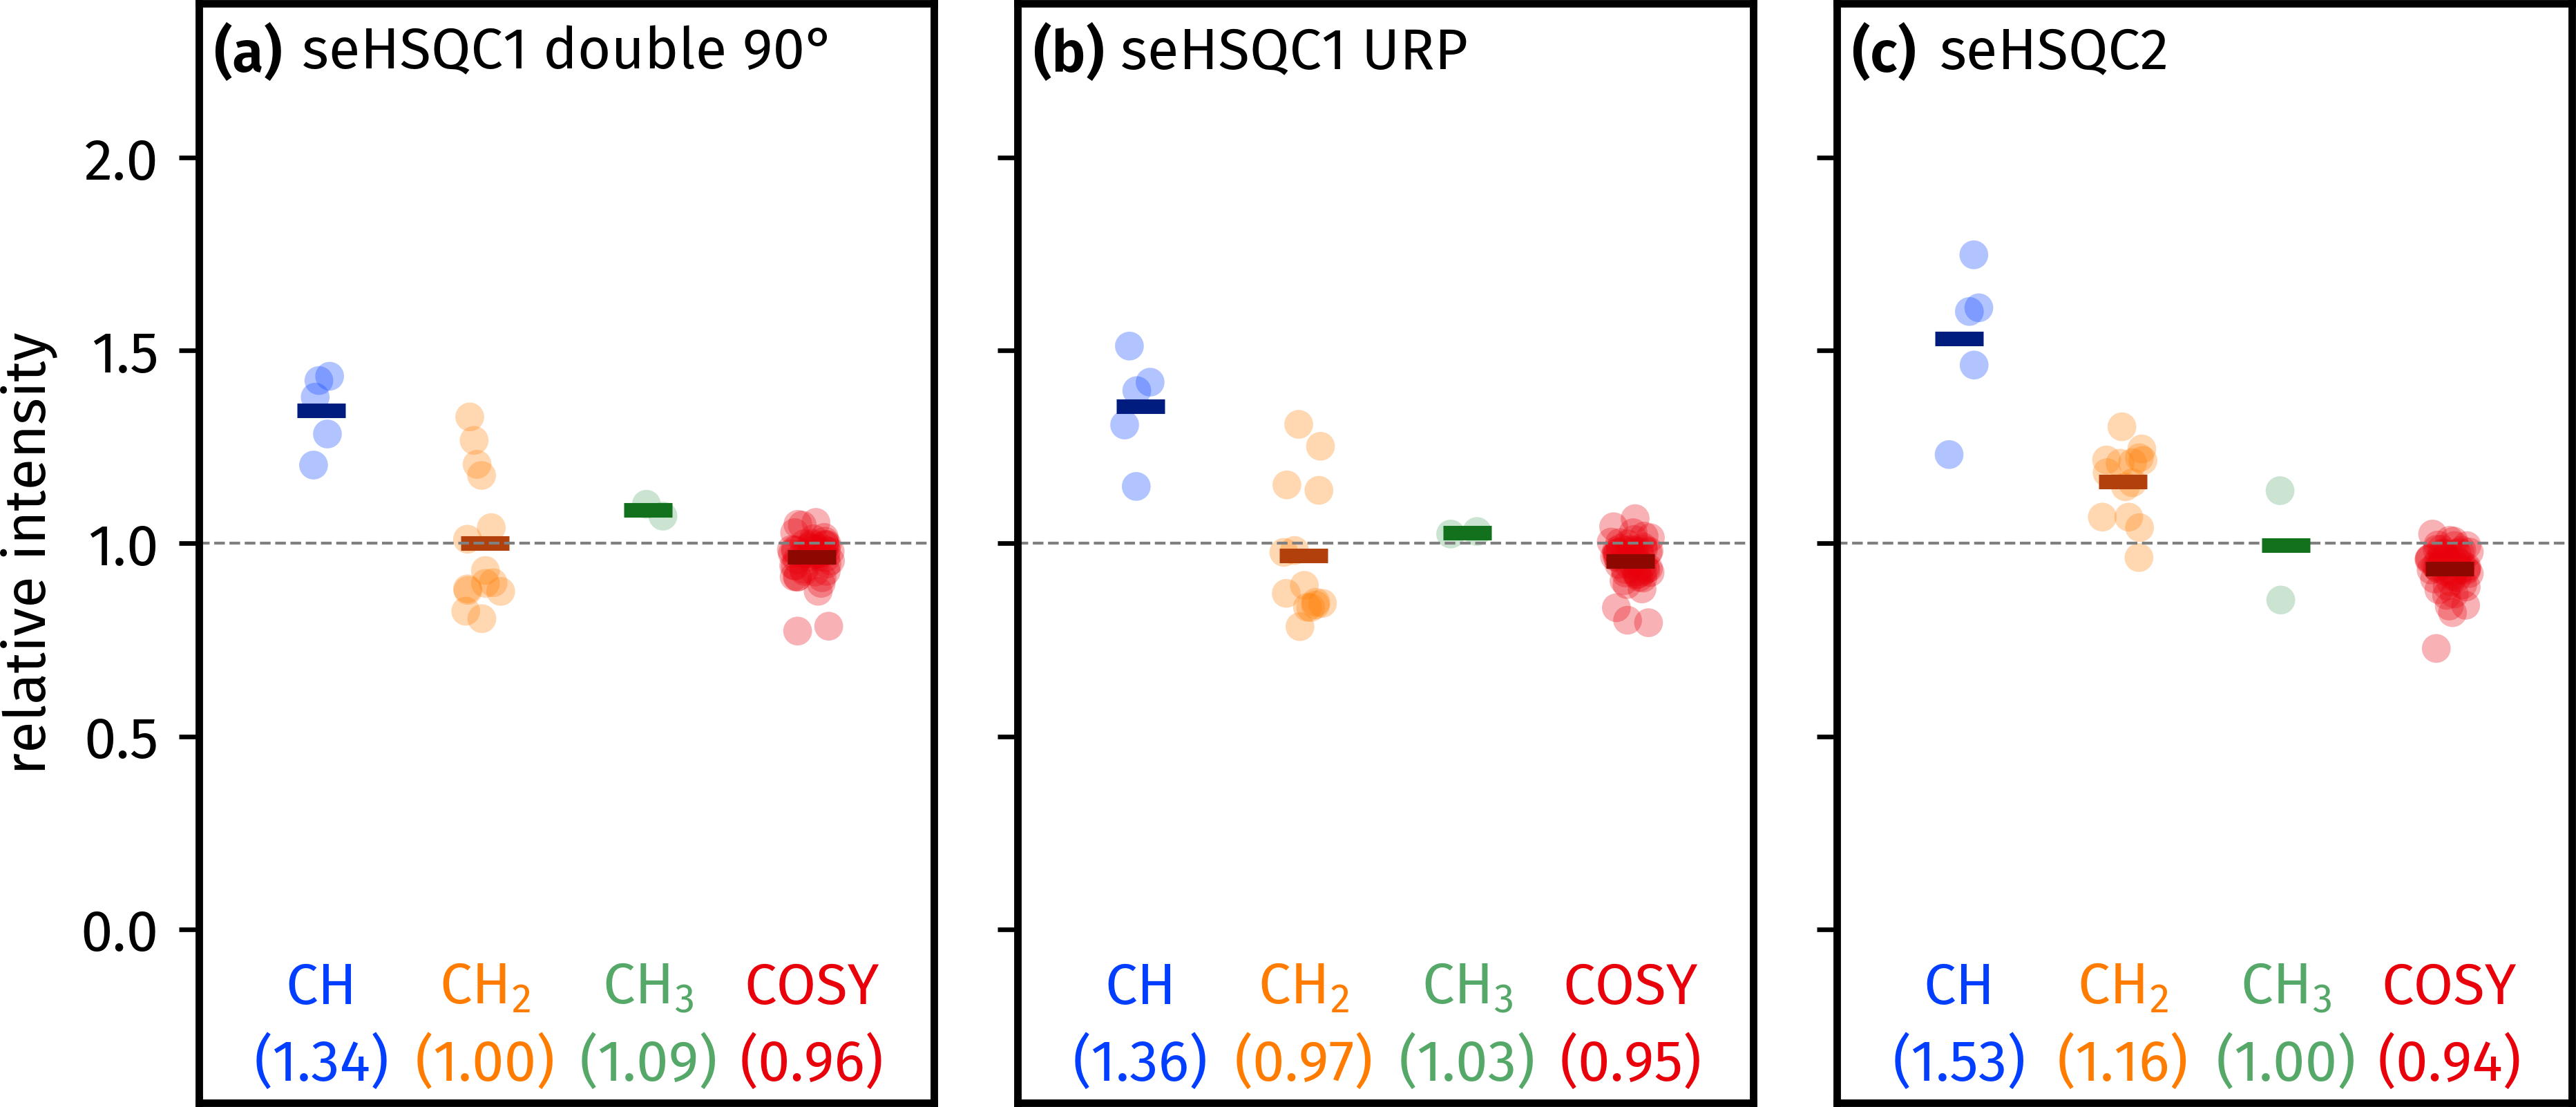
\includegraphics[draft=false]{noah/sehsqc1_urp_sens.png}%
    {\phantomsubcaption\label{fig:sehsqc1_urp_sens_1dp}}%
    {\phantomsubcaption\label{fig:sehsqc1_urp_sens_1urp}}%
    {\phantomsubcaption\label{fig:sehsqc1_urp_sens_2}}%
    \caption[Sensitivity comparison of seHSQC1 module with URP]{
        Sensitivity comparisons using the seHSQC1 URP.
        $\Delta'$ was set to $1 / (8 \cdot \oneJ{CH})$; no multiplicity editing was used.
        Note that a different dataset was used for this figure and \cref{fig:noah_sehsqc_comp}, so the numbers are very slightly different.
        \textbf{(\subref{fig:sehsqc1_urp_sens_1dp})} Original seHSQC1 module with double \proton{} \ang{90} pulse.
        \textbf{(\subref{fig:sehsqc1_urp_sens_1urp})} seHSQC1 using the optimised URP shown in \cref{fig:spv1_urp_magn}.
        \textbf{(\subref{fig:sehsqc1_urp_sens_2})} seHSQC2 module for comparison.
        \datacode{7A-220110}
    }
    \label{fig:sehsqc1_urp_sens}
\end{figure}


\subsubsection{BIG-BIRD versus ZIP}

The final point in this section pertains to the implementation of the seHSQC2 module.
As it stands, the isotope-specific rotation element placed at the start of the module is the ZIP element: its role is to effect \ang{90} rotations with different phases on the \magn{C} and \magnnot{C} magnetisation pools.
However, such pulse elements have been known for a long time: these include TANGO\autocite{Wimperis1984JMR}, BANGO\autocite{Sorensen1994BMR}, BIRD\autocite{Garbow1982CPL,Uhrin1993JMRSA,Kaltschnee2014CC}, BIG-BIRD\autocite{Briand1997JMR}, and TIG-BIRD\autocite{Briand1998JMR}.
In particular, the BIG-BIRD element can be designed to accomplish the same overall effect as the ZIP element.
For the seHSQC2 without multiplicity editing, we can therefore replace the ZIP element with
\begin{equation}
    \label{eq:big_bird_unedited}
    45\rlap{\unit{\degree}}_{\ang{45}}(\proton{})\text{--}2\Delta\text{--}\ang{180}(\proton{},\carbon{})\text{--}2\Delta\text{--}45\rlap{\unit{\degree}}_{\ang{225}}(\proton{}),
\end{equation}
where $\beta_\phi$ represents a hard pulse with flip angle $\beta$ and phase $\phi$.
For the edited seHSQC, the phases must be altered slightly:
\begin{equation}
    \label{eq:big_bird_edited}
    45\rlap{\unit{\degree}}_{\ang{315}}(\proton{})\text{--}2\Delta\text{--}\ang{180}(\proton{},\carbon{})\text{--}2\Delta\text{--}45\rlap{\unit{\degree}}_{\ang{135}}(\proton{}).
\end{equation}
This BIG-BIRD version of the seHSQC2 was also evaluated.
However, its performance in all respects was not as good as the ZIP version: both the seHSQC sensitivity itself, as well as the sensitivity of the later CLIP-COSY, were lower when the BIG-BIRD element was used.

\begin{figure}[!ht]
    \centering
    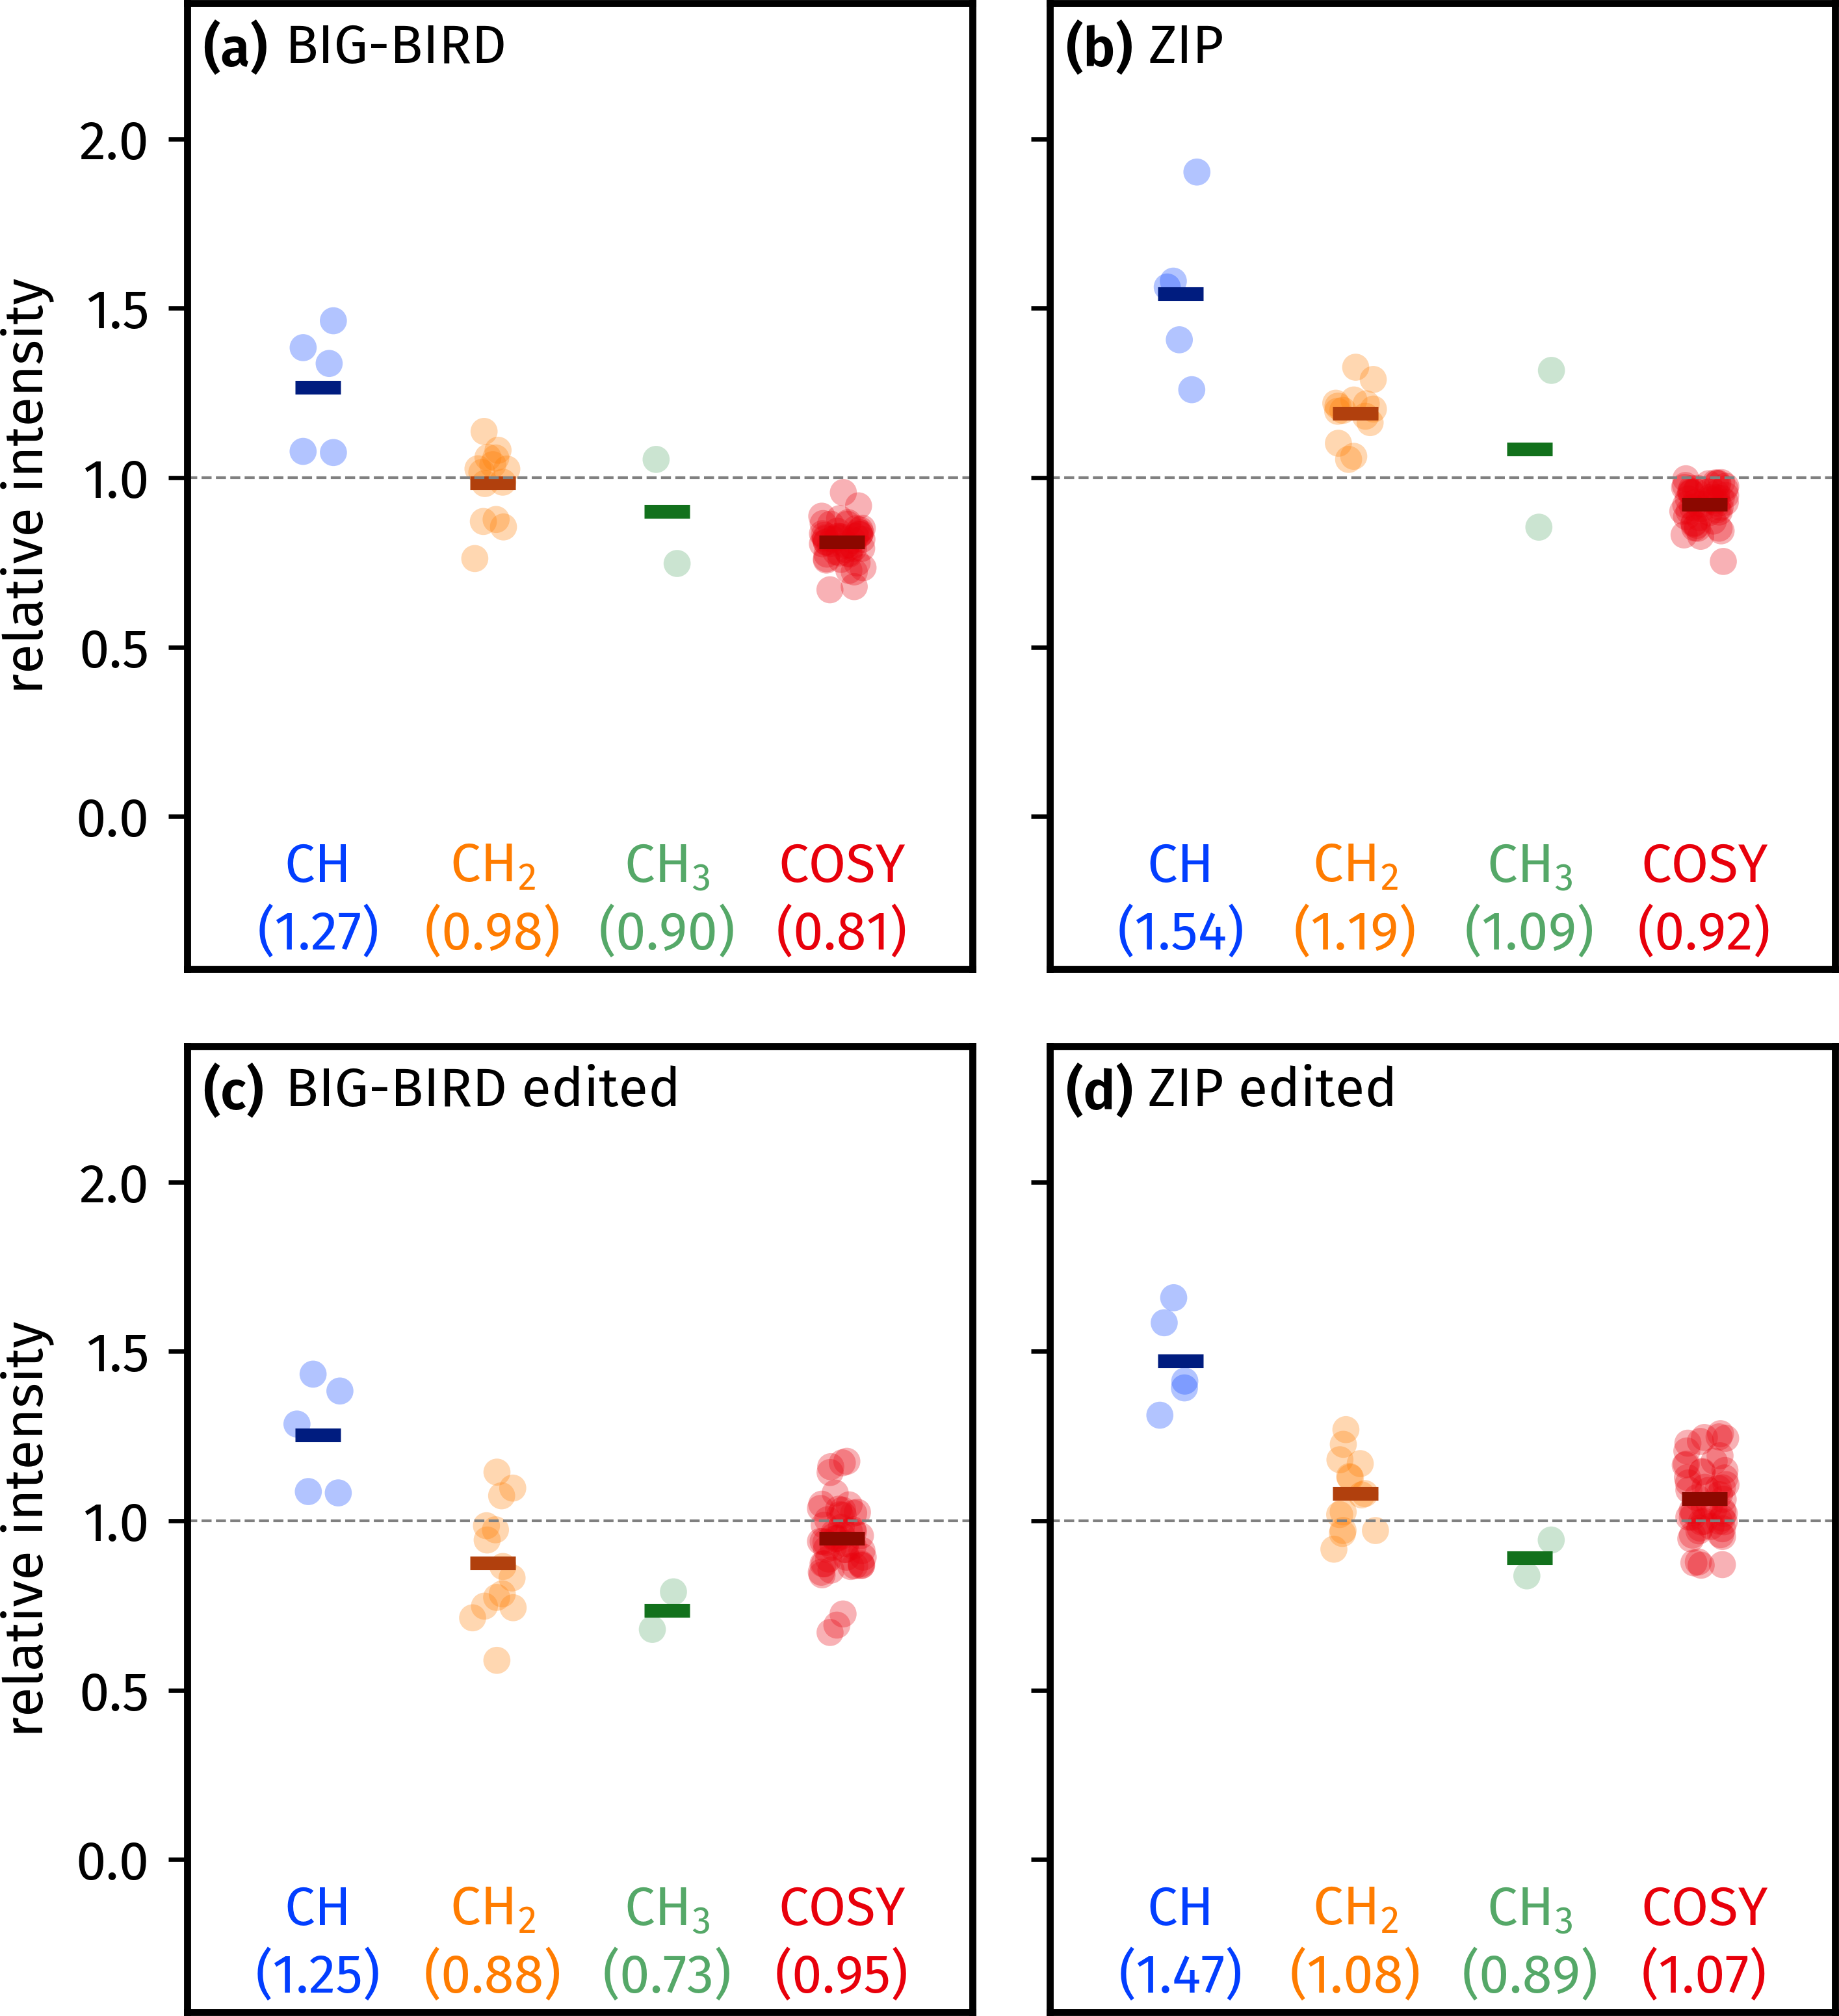
\includegraphics[draft=false]{noah/sehsqc_bigbird.png}%
    {\phantomsubcaption\label{fig:noah_sehsqc_bigbird_bb_noed}}%
    {\phantomsubcaption\label{fig:noah_sehsqc_bigbird_zip_noed}}%
    {\phantomsubcaption\label{fig:noah_sehsqc_bigbird_bb_ed}}%
    {\phantomsubcaption\label{fig:noah_sehsqc_bigbird_zip_ed}}%
    \caption[Comparison of BIG-BIRD and ZIP pulse elements in seHSQC2 module]{
        Sensitivity comparisons of BIG-BIRD and ZIP pulse elements in seHSQC2 module.
        The reference dataset being compared against is still the \noah{S,Cc} (but with editing in (\subref{fig:noah_sehsqc_bigbird_bb_ed}) and (\subref{fig:noah_sehsqc_bigbird_zip_ed}).
        The delay $\Delta'$ was set to $1 / (8 \cdot \oneJ{CH})$.
        \textbf{(\subref{fig:noah_sehsqc_bigbird_bb_noed})} Unedited seHSQC2 using BIG-BIRD.
        \textbf{(\subref{fig:noah_sehsqc_bigbird_zip_noed})} Unedited seHSQC2 using ZIP.
        \textbf{(\subref{fig:noah_sehsqc_bigbird_bb_ed})} Edited seHSQC2 using BIG-BIRD.
        \textbf{(\subref{fig:noah_sehsqc_bigbird_zip_ed})} Edited seHSQC2 using ZIP.
        \datacode{7A-201115}
    }
    \label{fig:noah_sehsqc_bigbird}
\end{figure}
